\documentclass[aspectratio=169,11pt]{beamer}

\usepackage[T1]{fontenc}
\usepackage[utf8]{inputenc}
\usepackage[sfdefault]{FiraSans}
\usefonttheme{professionalfonts}
\usepackage{amsmath}
\usepackage{booktabs}
\usepackage{graphicx}
\usepackage{tikz}
\usepackage{pgfplots}
\usepackage{appendixnumberbeamer}
\usepackage{csquotes}

\pgfplotsset{compat=1.18}
\usetikzlibrary{arrows.meta,calc,fit,positioning,shapes.geometric}
\setbeameroption{hide notes}

\definecolor{td3navy}{HTML}{15304A}
\definecolor{td3teal}{HTML}{0D6E6E}
\definecolor{td3gold}{HTML}{D49A32}
\definecolor{td3bg}{HTML}{F5F7FA}
\definecolor{td3muted}{HTML}{5F6B7A}
\definecolor{td3soft}{HTML}{EAF1F6}
\definecolor{td3green}{HTML}{2E7D5A}
\definecolor{td3red}{HTML}{B04A4A}

\setbeamercolor{background canvas}{bg=white}
\setbeamercolor{normal text}{fg=td3navy,bg=white}
\setbeamercolor{structure}{fg=td3teal}
\setbeamercolor{frametitle}{fg=white,bg=td3navy}
\setbeamercolor{title}{fg=td3navy}
\setbeamercolor{subtitle}{fg=td3muted}
\setbeamercolor{block title}{fg=white,bg=td3teal}
\setbeamercolor{block body}{fg=td3navy,bg=td3soft}
\setbeamercolor{alerted text}{fg=td3gold}
\setbeamercolor{itemize item}{fg=td3gold}
\setbeamercolor{itemize subitem}{fg=td3gold}

\setbeamertemplate{navigation symbols}{}
\setbeamertemplate{footline}[frame number]
\setbeamertemplate{itemize item}{\large$\blacktriangleright$}
\setbeamertemplate{itemize subitem}{\small$\bullet$}
\setbeamertemplate{blocks}[rounded][shadow=false]
\setbeamersize{text margin left=1.0cm,text margin right=1.0cm}

\setbeamerfont{title}{size=\LARGE,series=\bfseries}
\setbeamerfont{subtitle}{size=\large}
\setbeamerfont{author}{size=\large}
\setbeamerfont{date}{size=\normalsize}
\setbeamerfont{frametitle}{size=\Large,series=\bfseries}
\setbeamerfont{normal text}{size=\large}
\setbeamerfont{block title}{size=\large,series=\bfseries}
\setbeamerfont{block body}{size=\normalsize}

\newlength{\sourceboxheight}
\setlength{\sourceboxheight}{1.15cm}
\newlength{\sourcebottomgap}
\setlength{\sourcebottomgap}{0.38cm}
\newcommand{\source}[1]{%
  \par\vspace*{\sourceboxheight}%
  \begin{tikzpicture}[remember picture,overlay]
    \node[
      anchor=south west,
      inner sep=0pt,
      text width=\dimexpr\paperwidth-2cm\relax,
      align=left
    ] at ([xshift=1cm,yshift=\sourcebottomgap]current page.south west) {%
      \raggedright\footnotesize\color{td3muted}#1%
    };
  \end{tikzpicture}%
}
\newcommand{\good}{\textcolor{td3green}{\textbf{Strength}}}
\newcommand{\bad}{\textcolor{td3red}{\textbf{Limitation}}}
\newcommand{\reflink}[2]{\href{#1}{\textcolor{td3teal}{\texttt{#2}}}}
\newcommand{\panelbox}[2]{%
  \begin{block}{#1}
    \raggedright
    #2
  \end{block}
}
\newenvironment{twopanelrow}{\begin{columns}[T,onlytextwidth]}{\end{columns}}
\newenvironment{threepanelrow}{\begin{columns}[T,onlytextwidth]}{\end{columns}}
\newcommand{\twopanel}[2]{\column{0.480\textwidth}\panelbox{#1}{#2}}
\newcommand{\threepanel}[2]{\column{0.305\textwidth}\panelbox{#1}{#2}}

\title{Who Hunts Who?}
\subtitle{Comparing Four Knowledge Graph Construction Methods\\for Predator–Prey Relations}
\author{[Author Names]}
\institute{Natural Language Processing}
\date{June 2026}

% ─────────────────────────────────────────────────────────────────────────────
\begin{document}
% ─────────────────────────────────────────────────────────────────────────────

\begin{frame}[plain]
  \titlepage
  \note{
    Introduce the project: we built a predator--prey knowledge graph from
    Wikipedia text and compared four extraction methods. The talk walks through
    the design of each method, then compares them on a shared gold standard.
  }
\end{frame}

% ─── MOTIVATION ──────────────────────────────────────────────────────────────

\begin{frame}{Motivation \& Task}
  \begin{columns}[T,totalwidth=\textwidth]
    \column{0.56\textwidth}
      \begin{itemize}
        \item Goal: automatically build a \alert{predator--prey knowledge graph} from free text.
        \item Source: Wikipedia pages for 18 animals across three trophic levels.
        \item No animal-specific hand-written rules --- only general NLP signals.
        \item Central question: \alert{which extraction approach yields the best trade-off between precision and recall?}
      \end{itemize}
    \column{0.40\textwidth}
      \begin{block}{Three trophic levels}
        \small
        \textbf{\textcolor{td3red}{Top predators (6)}} \\
        Hawk, Eagle, Barn Owl, Fox, Wolf, Weasel \\[0.45em]
        \textbf{\textcolor{td3gold}{Mid-level (4)}} \\
        Salamander, Lizard, Spider, Bat \\[0.45em]
        \textbf{\textcolor{td3green}{Prey (8)}} \\
        Mouse, Rabbit, Squirrel,\\
        Grasshopper, Cricket,\\
        Caterpillar, Fly, Beetle
      \end{block}
  \end{columns}
  \note{
    Stress the point that we deliberately chose animals whose Wikipedia pages
    contain explicit predation statements -- this is a controlled setup that
    lets us evaluate NLP methods cleanly.
  }
\end{frame}

% ─── PIPELINE ────────────────────────────────────────────────────────────────

\begin{frame}{Pipeline Overview}
  \centering
  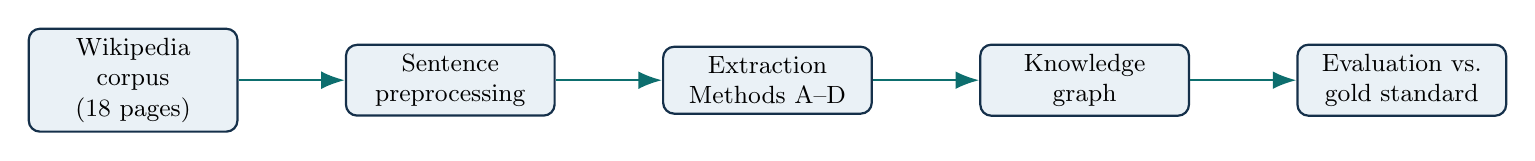
\begin{tikzpicture}[
    node distance=0.45cm and 1.35cm,
    box/.style={rounded corners, draw=td3navy, thick, fill=td3soft,
                minimum width=2.65cm, minimum height=0.85cm,
                align=center, font=\small},
    arrow/.style={-{Latex[length=3mm]}, thick, color=td3teal}
  ]
    \node[box] (wiki)     {Wikipedia\\corpus\\(18 pages)};
    \node[box, right=of wiki]     (pre)  {Sentence\\preprocessing};
    \node[box, right=of pre]      (extr) {Extraction\\Methods A--D};
    \node[box, right=of extr]     (graph){Knowledge\\graph};
    \node[box, right=of graph]    (eval) {Evaluation vs.\\gold standard};
    \draw[arrow] (wiki) -- (pre);
    \draw[arrow] (pre)  -- (extr);
    \draw[arrow] (extr) -- (graph);
    \draw[arrow] (graph)-- (eval);
  \end{tikzpicture}

  \vspace{0.8em}
  \begin{threepanelrow}
    \threepanel{Corpus}{
      \small Pages fetched via \texttt{wikipedia-api}, cached as JSON.
      Text is stripped of markup, parentheticals, and citation markers, then split into sentences.
    }
    \threepanel{Gold standard}{
      \small 38 manually curated predator$\to$prey edges.
      The same benchmark is used for all four methods to ensure a fair comparison.
    }
    \threepanel{Metrics}{
      \small Edge-level Precision, Recall, and F1 score.
      Only edges within valid trophic directions are considered.
    }
  \end{threepanelrow}
  \note{
    Walk through the pipeline once before diving into the methods.
    Emphasise that the evaluation is held constant across all methods.
  }
\end{frame}

% ─── GOLD STANDARD ───────────────────────────────────────────────────────────

\begin{frame}{Gold Standard}
  \begin{twopanelrow}
    \twopanel{Construction rules}{
      \small
      \begin{itemize}
        \item Manually verified from Wikipedia text and biological knowledge.
        \item Only directed edges: predator $\to$ prey.
        \item Trophic constraints enforced:
          \begin{itemize}
            \item top predators may target mid-level \emph{and} prey.
            \item mid-level predators may target prey only.
          \end{itemize}
        \item 38 edges in total across 10 source animals.
      \end{itemize}
    }
    \twopanel{Gold standard graph}{
      \centering
      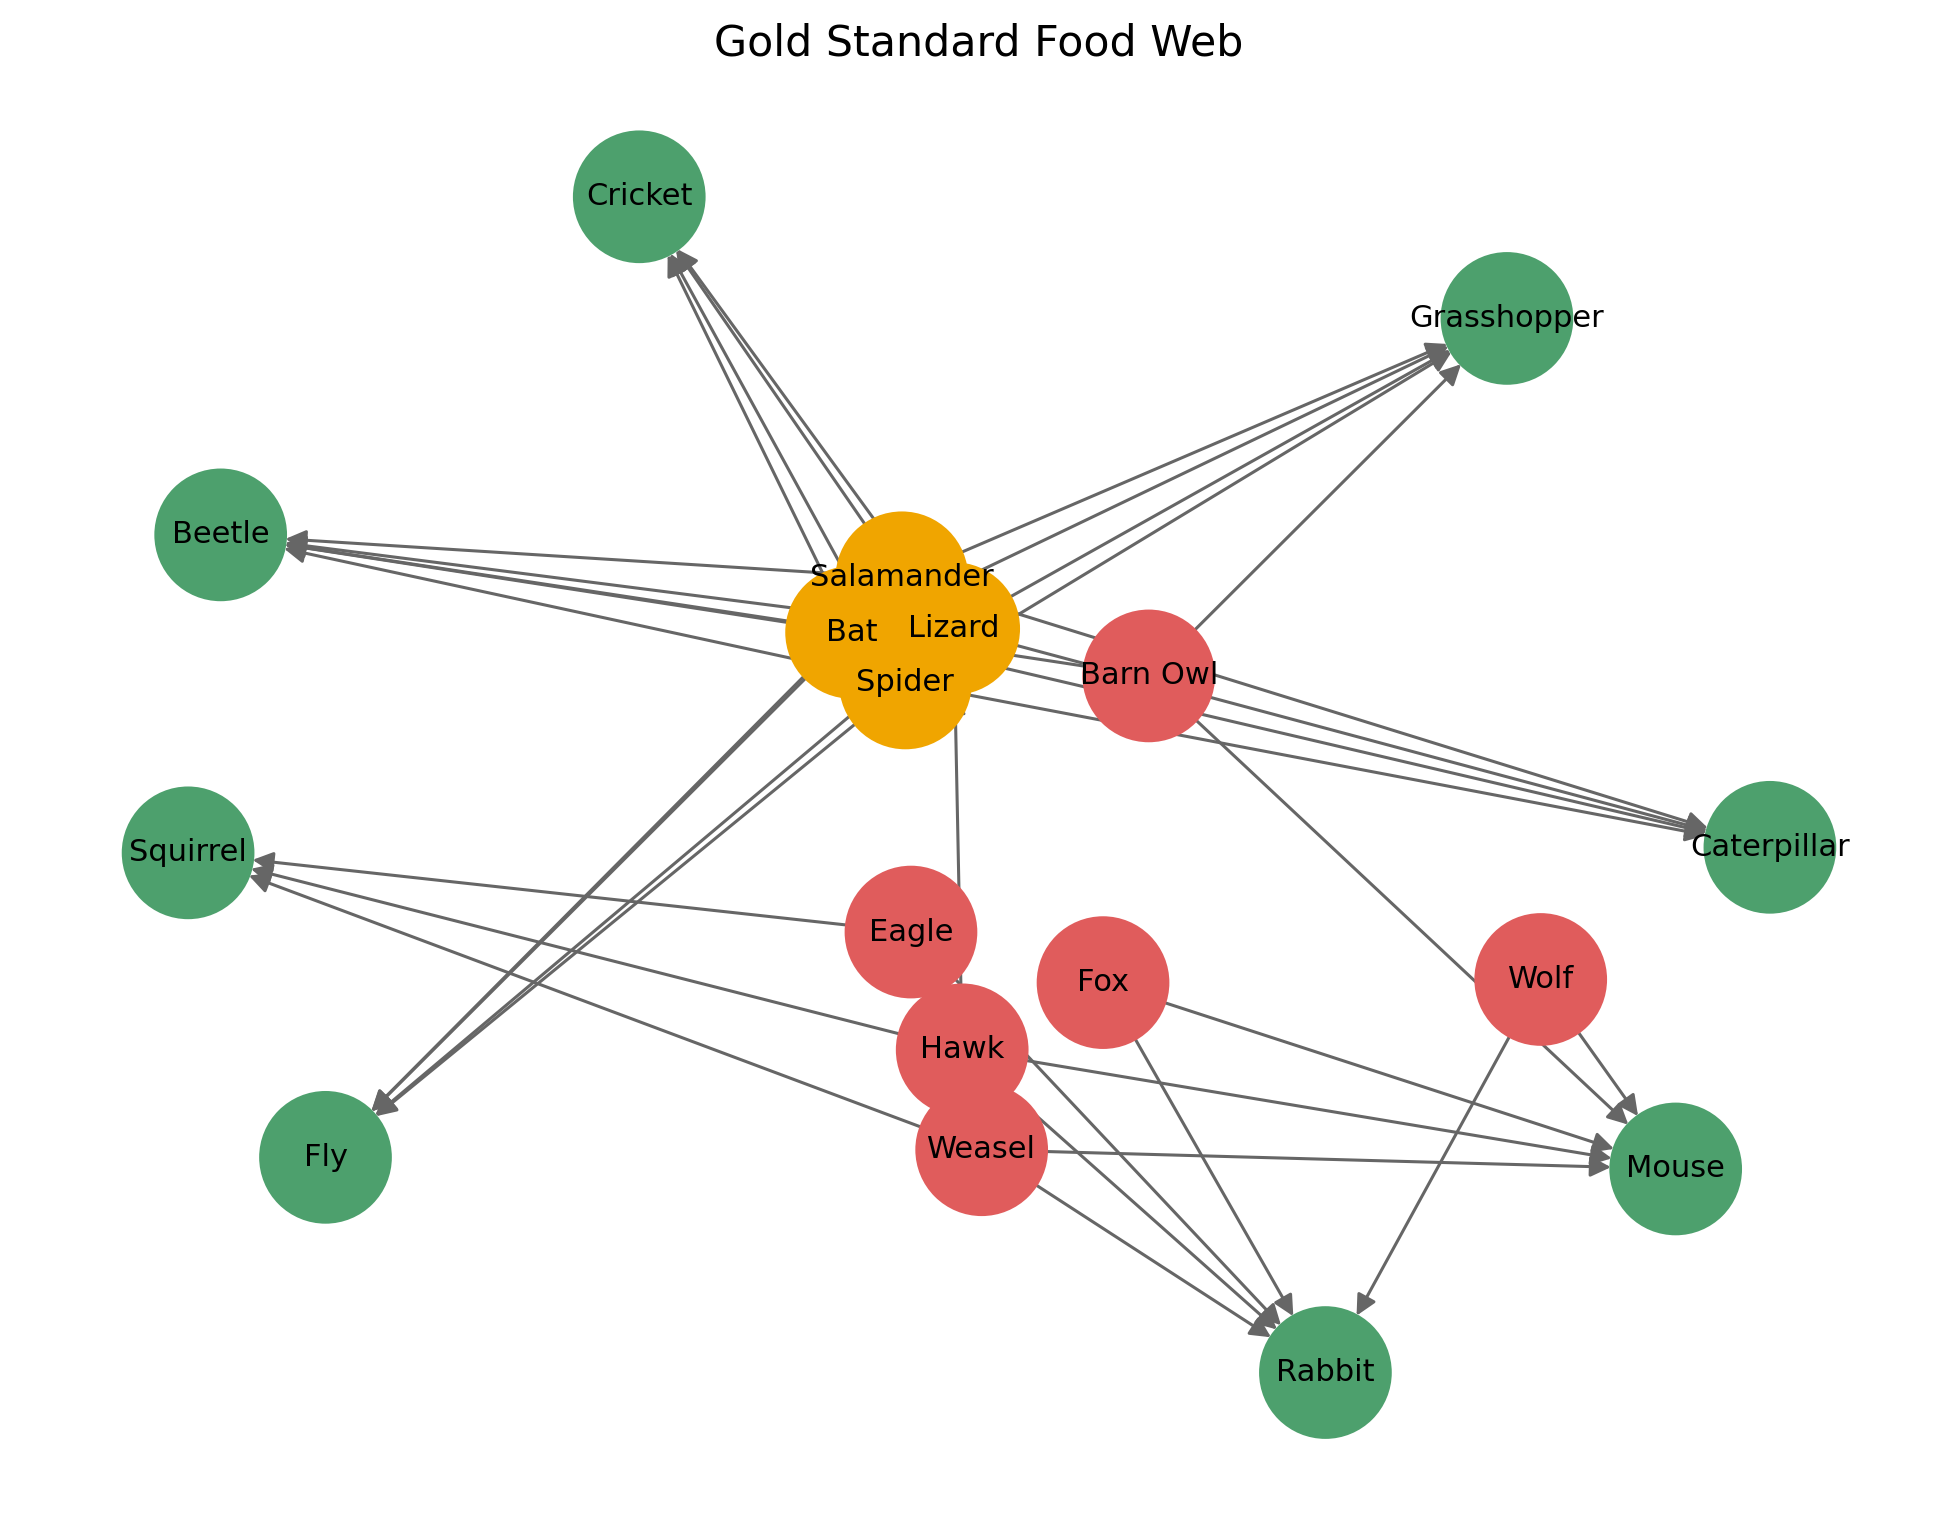
\includegraphics[width=0.98\linewidth]{slides_assets/gold_standard_food_web.png}
    }
  \end{twopanelrow}
  \source{Gold standard constructed manually; animals selected from \texttt{who\_hunts\_who.ipynb} corpus.}
  \note{
    Briefly explain why the gold standard matters: it is the only fair way to
    compare methods that were designed with different precision--recall trade-offs
    in mind.
  }
\end{frame}

\begin{frame}{Method A vs Gold Standard}
  \begin{columns}[T,totalwidth=\textwidth]
    \column{0.49\textwidth}
      \centering
      \textbf{Gold standard}\\[0.3em]
      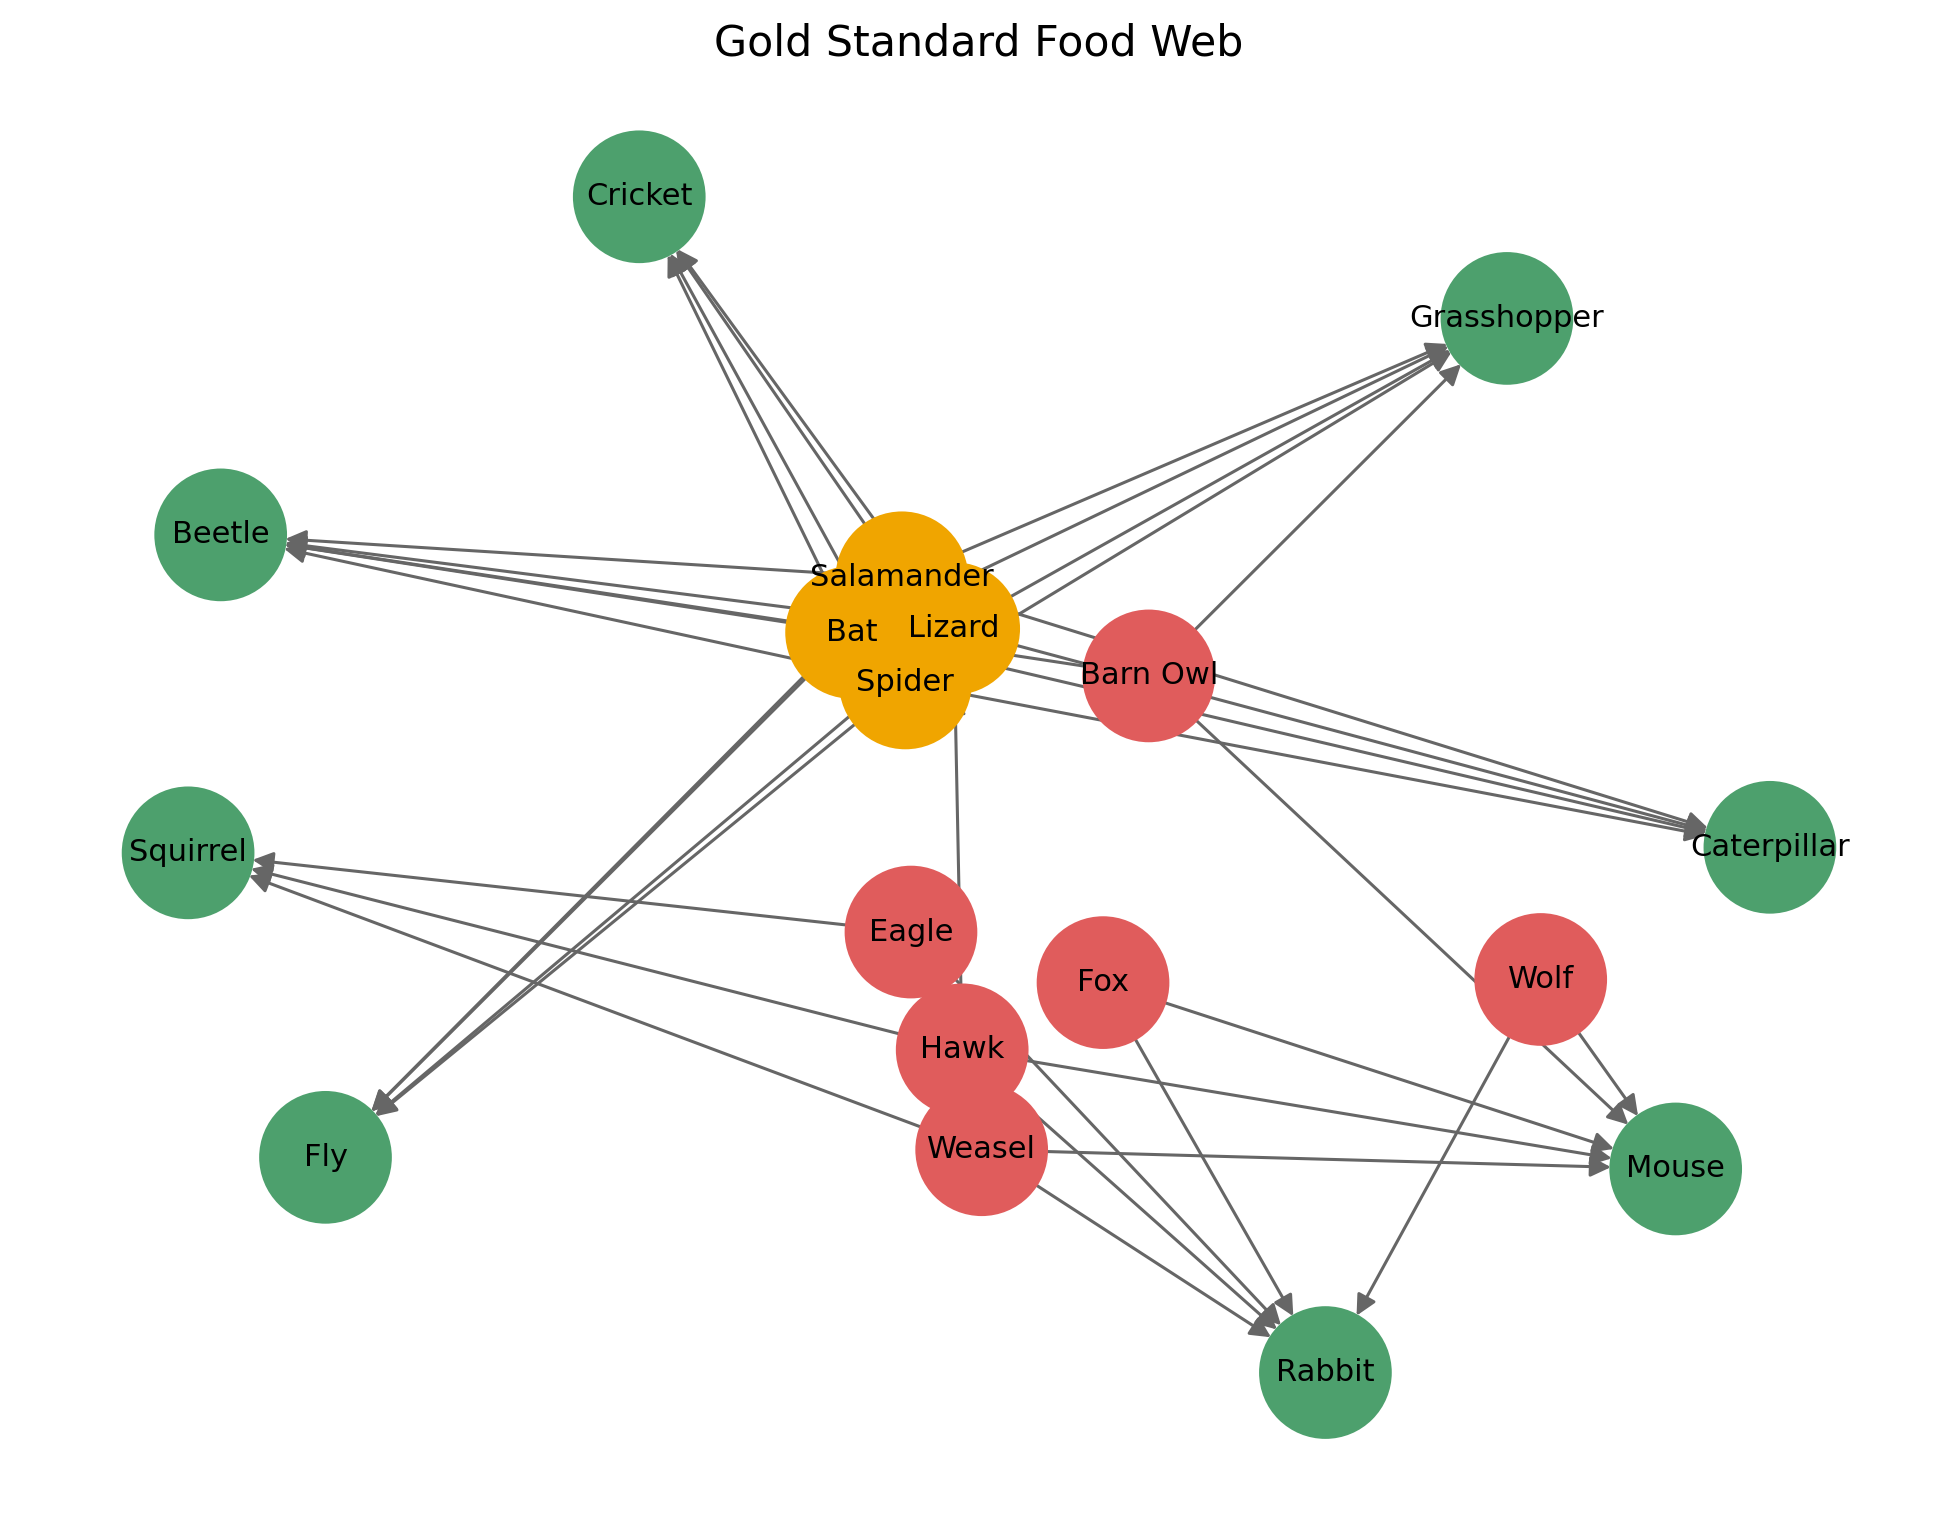
\includegraphics[width=\linewidth]{slides_assets/gold_standard_food_web.png}
    \column{0.49\textwidth}
      \centering
      \textbf{Method A}\\[0.3em]
      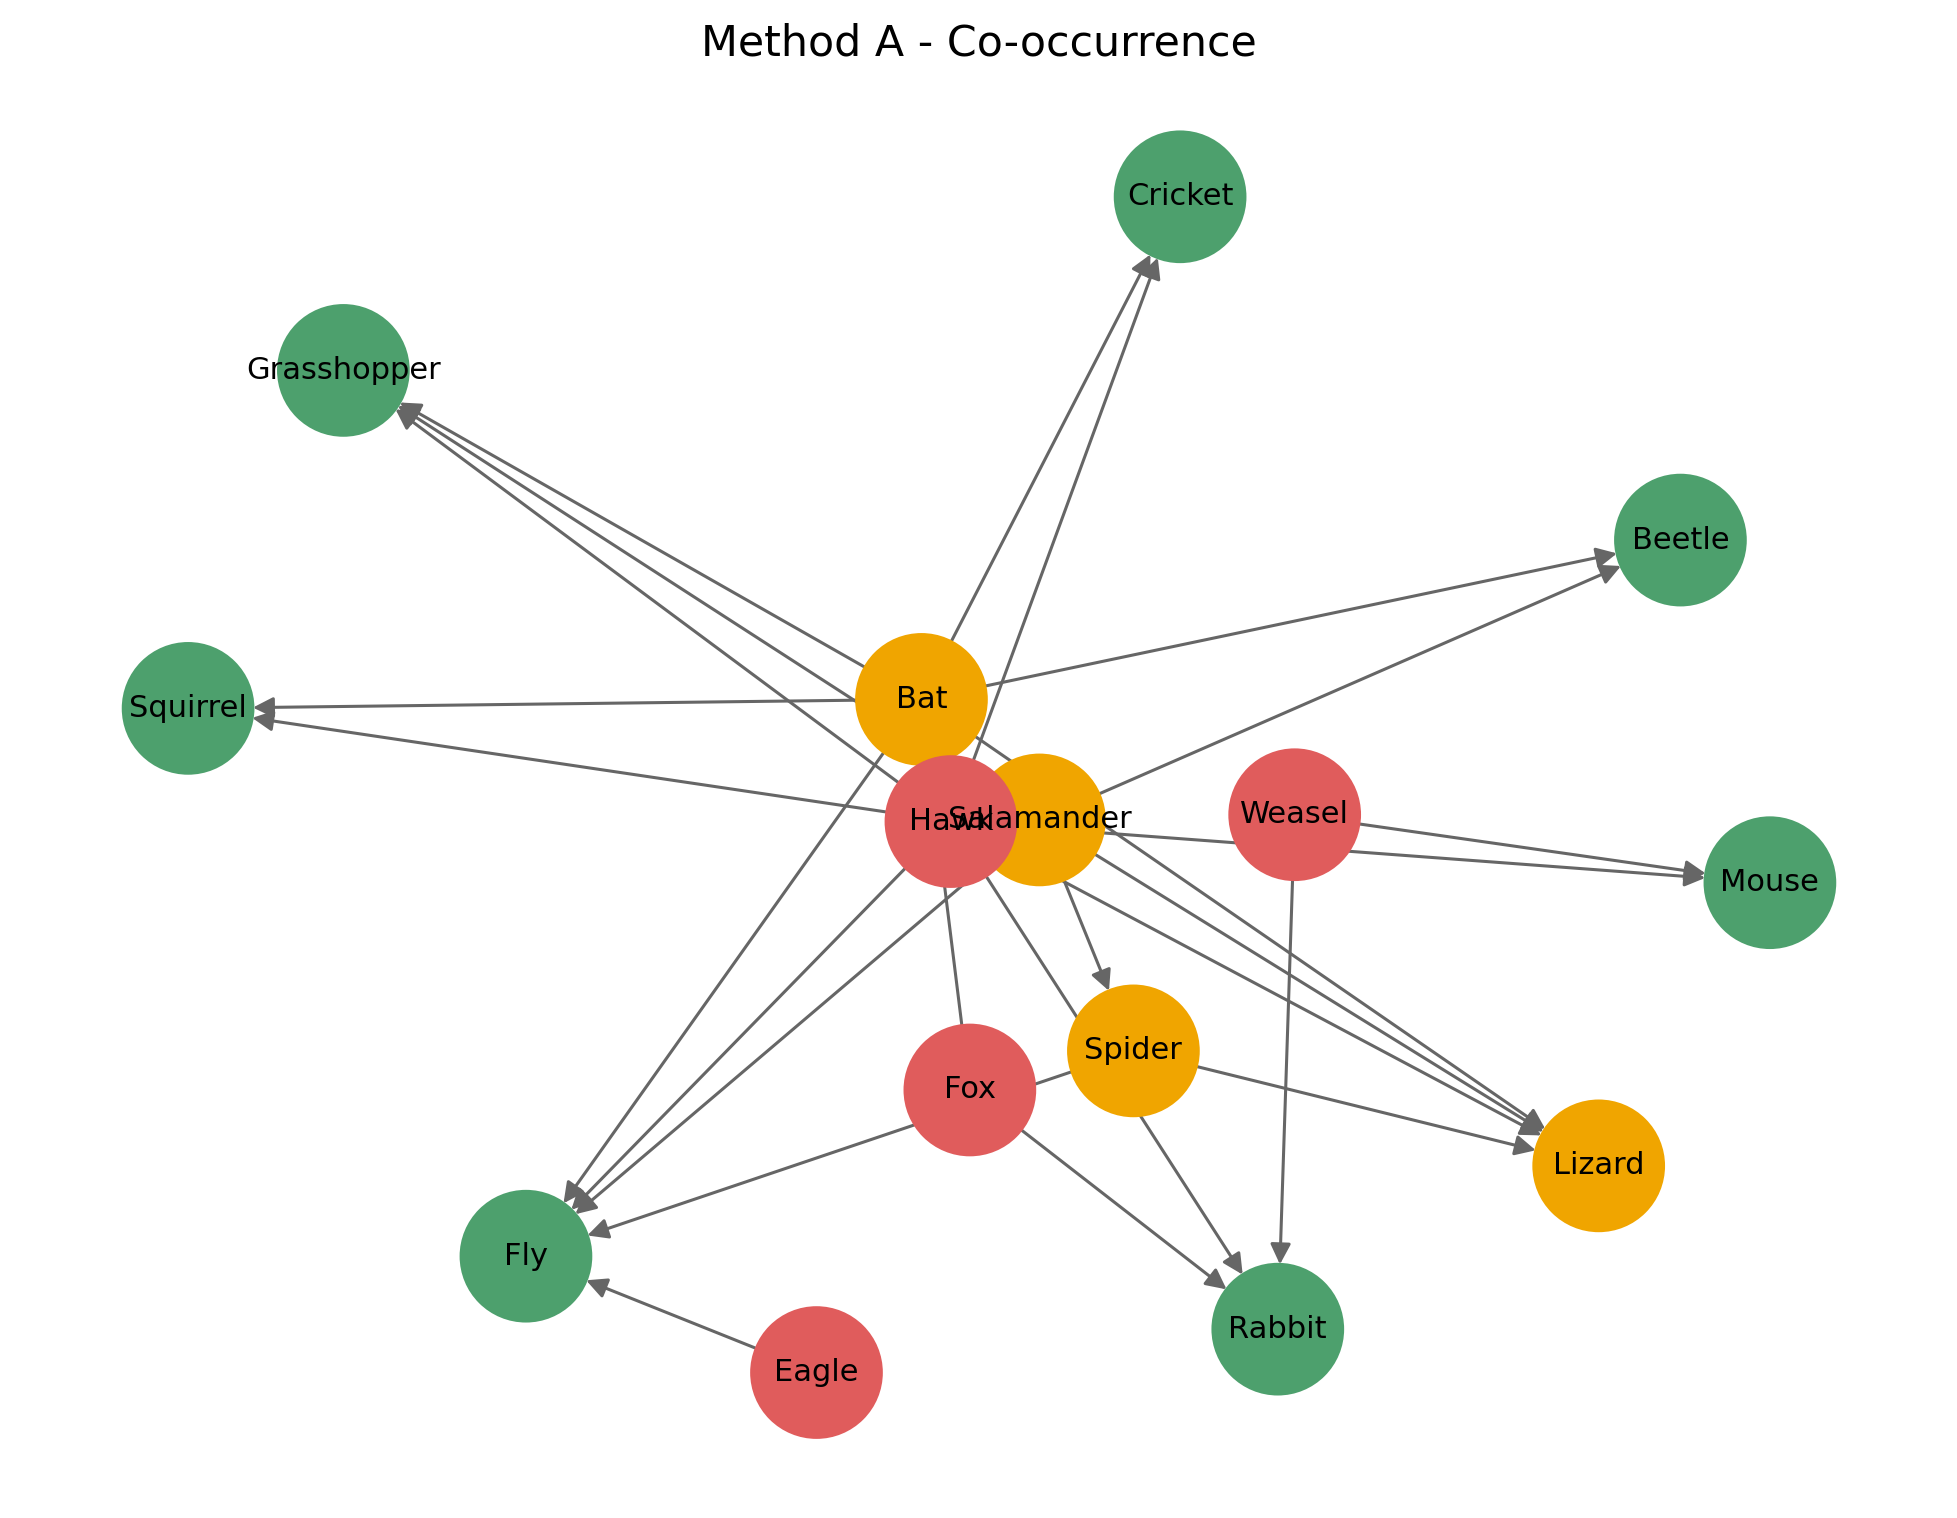
\includegraphics[width=\linewidth]{slides_assets/method_A_food_web.png}
  \end{columns}
  \vspace{0.4em}
  \begin{center}
    \small
    \textbf{Scores:} Precision $= 0.556$, Recall $= 0.278$, F1 $= 0.370$ \quad (TP $= 10$, FP $= 8$, FN $= 26$)
  \end{center}
\end{frame}

% ─── METHOD A ────────────────────────────────────────────────────────────────

\begin{frame}{Method A --- Co-occurrence}
  \begin{twopanelrow}
    \twopanel{How it works}{
      \small
      \begin{enumerate}
        \item For each source animal, iterate over sentences in its Wikipedia page.
        \item If any target animal is mentioned in the \alert{same sentence}: add edge source $\to$ target.
        \item No verb, no syntactic analysis --- pure proximity.
      \end{enumerate}
      \vspace{0.4em}
      \textbf{Example sentence:}\\
      \textit{``Hawks and foxes both compete for rabbits in open fields.''}\\[0.3em]
      $\Rightarrow$ adds Hawk$\to$Rabbit \emph{and} Fox$\to$Rabbit,\\
      \phantom{$\Rightarrow$ }even though the sentence is about \emph{competition}.
    }
    \twopanel{Design trade-offs}{
      \small
      \good: highest possible recall --- every real edge that co-occurs
      in a sentence will be found.

      \vspace{0.5em}
      \bad: no predation signal is required. Any two animals appearing
      together (as competitors, taxonomic relatives, or examples) become
      an edge.

      \vspace{0.5em}
      \bad: no direction inference --- edges are always assigned as
      source $\to$ target based on which page is being read.

      \vspace{0.5em}
      \textbf{Expected:} very high recall, low precision.
    }
  \end{twopanelrow}
  \note{
    Present Method A as the recall ceiling. Its result tells us how many gold
    edges are even textually accessible from these Wikipedia pages.
  }
\end{frame}

\begin{frame}{Method B vs Gold Standard}
  \begin{columns}[T,totalwidth=\textwidth]
    \column{0.49\textwidth}
      \centering
      \textbf{Gold standard}\\[0.3em]
      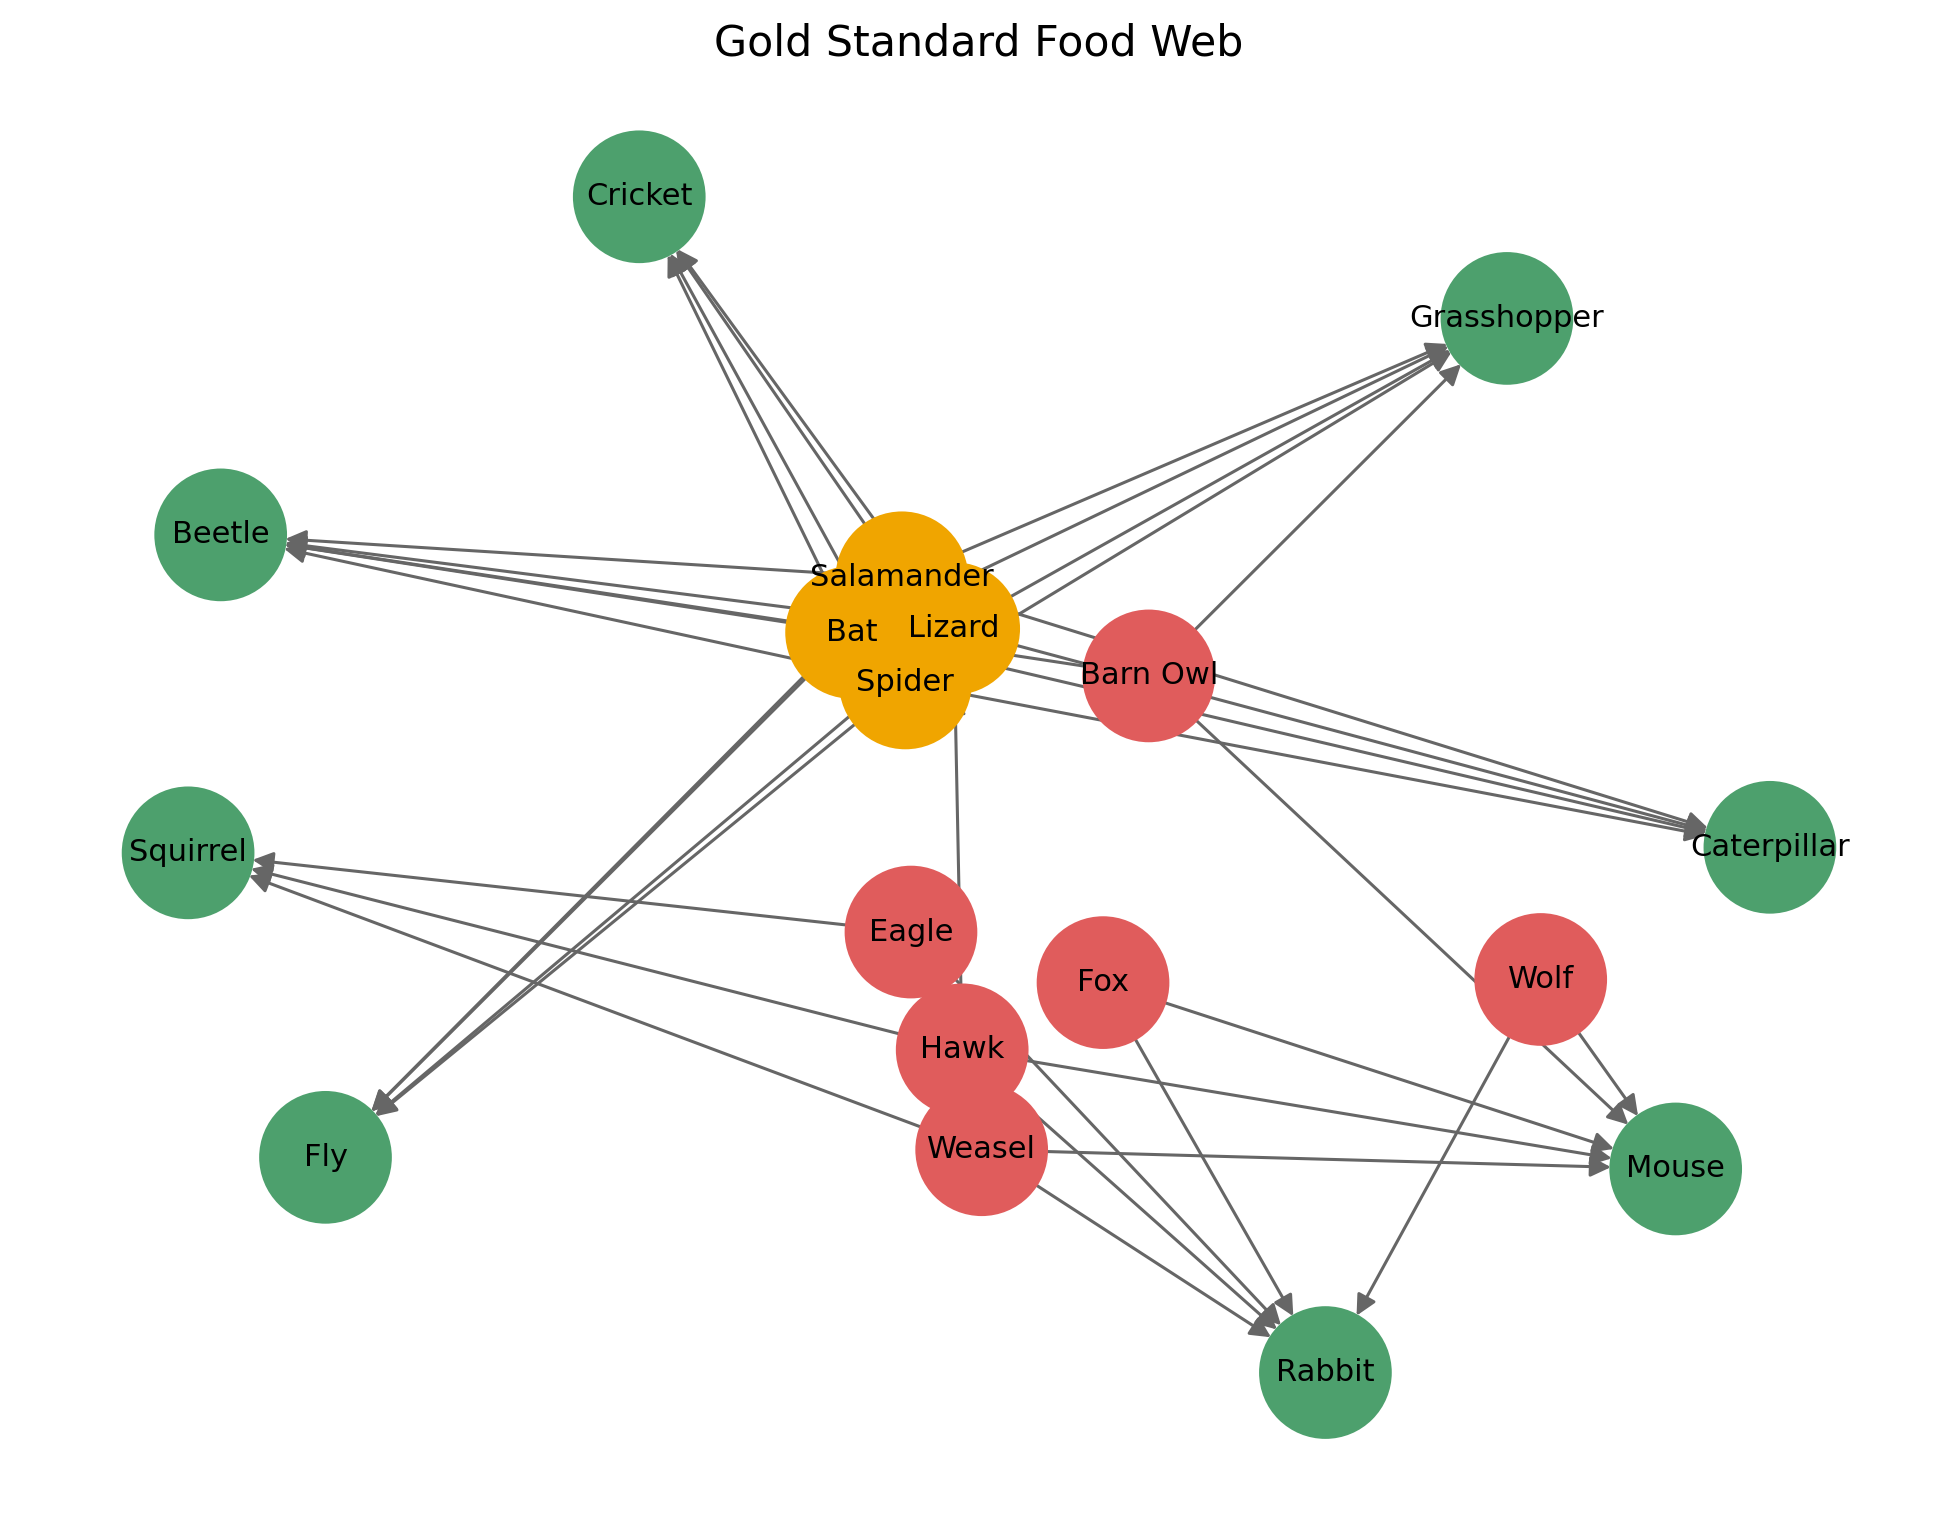
\includegraphics[width=\linewidth]{slides_assets/gold_standard_food_web.png}
    \column{0.49\textwidth}
      \centering
      \textbf{Method B}\\[0.3em]
      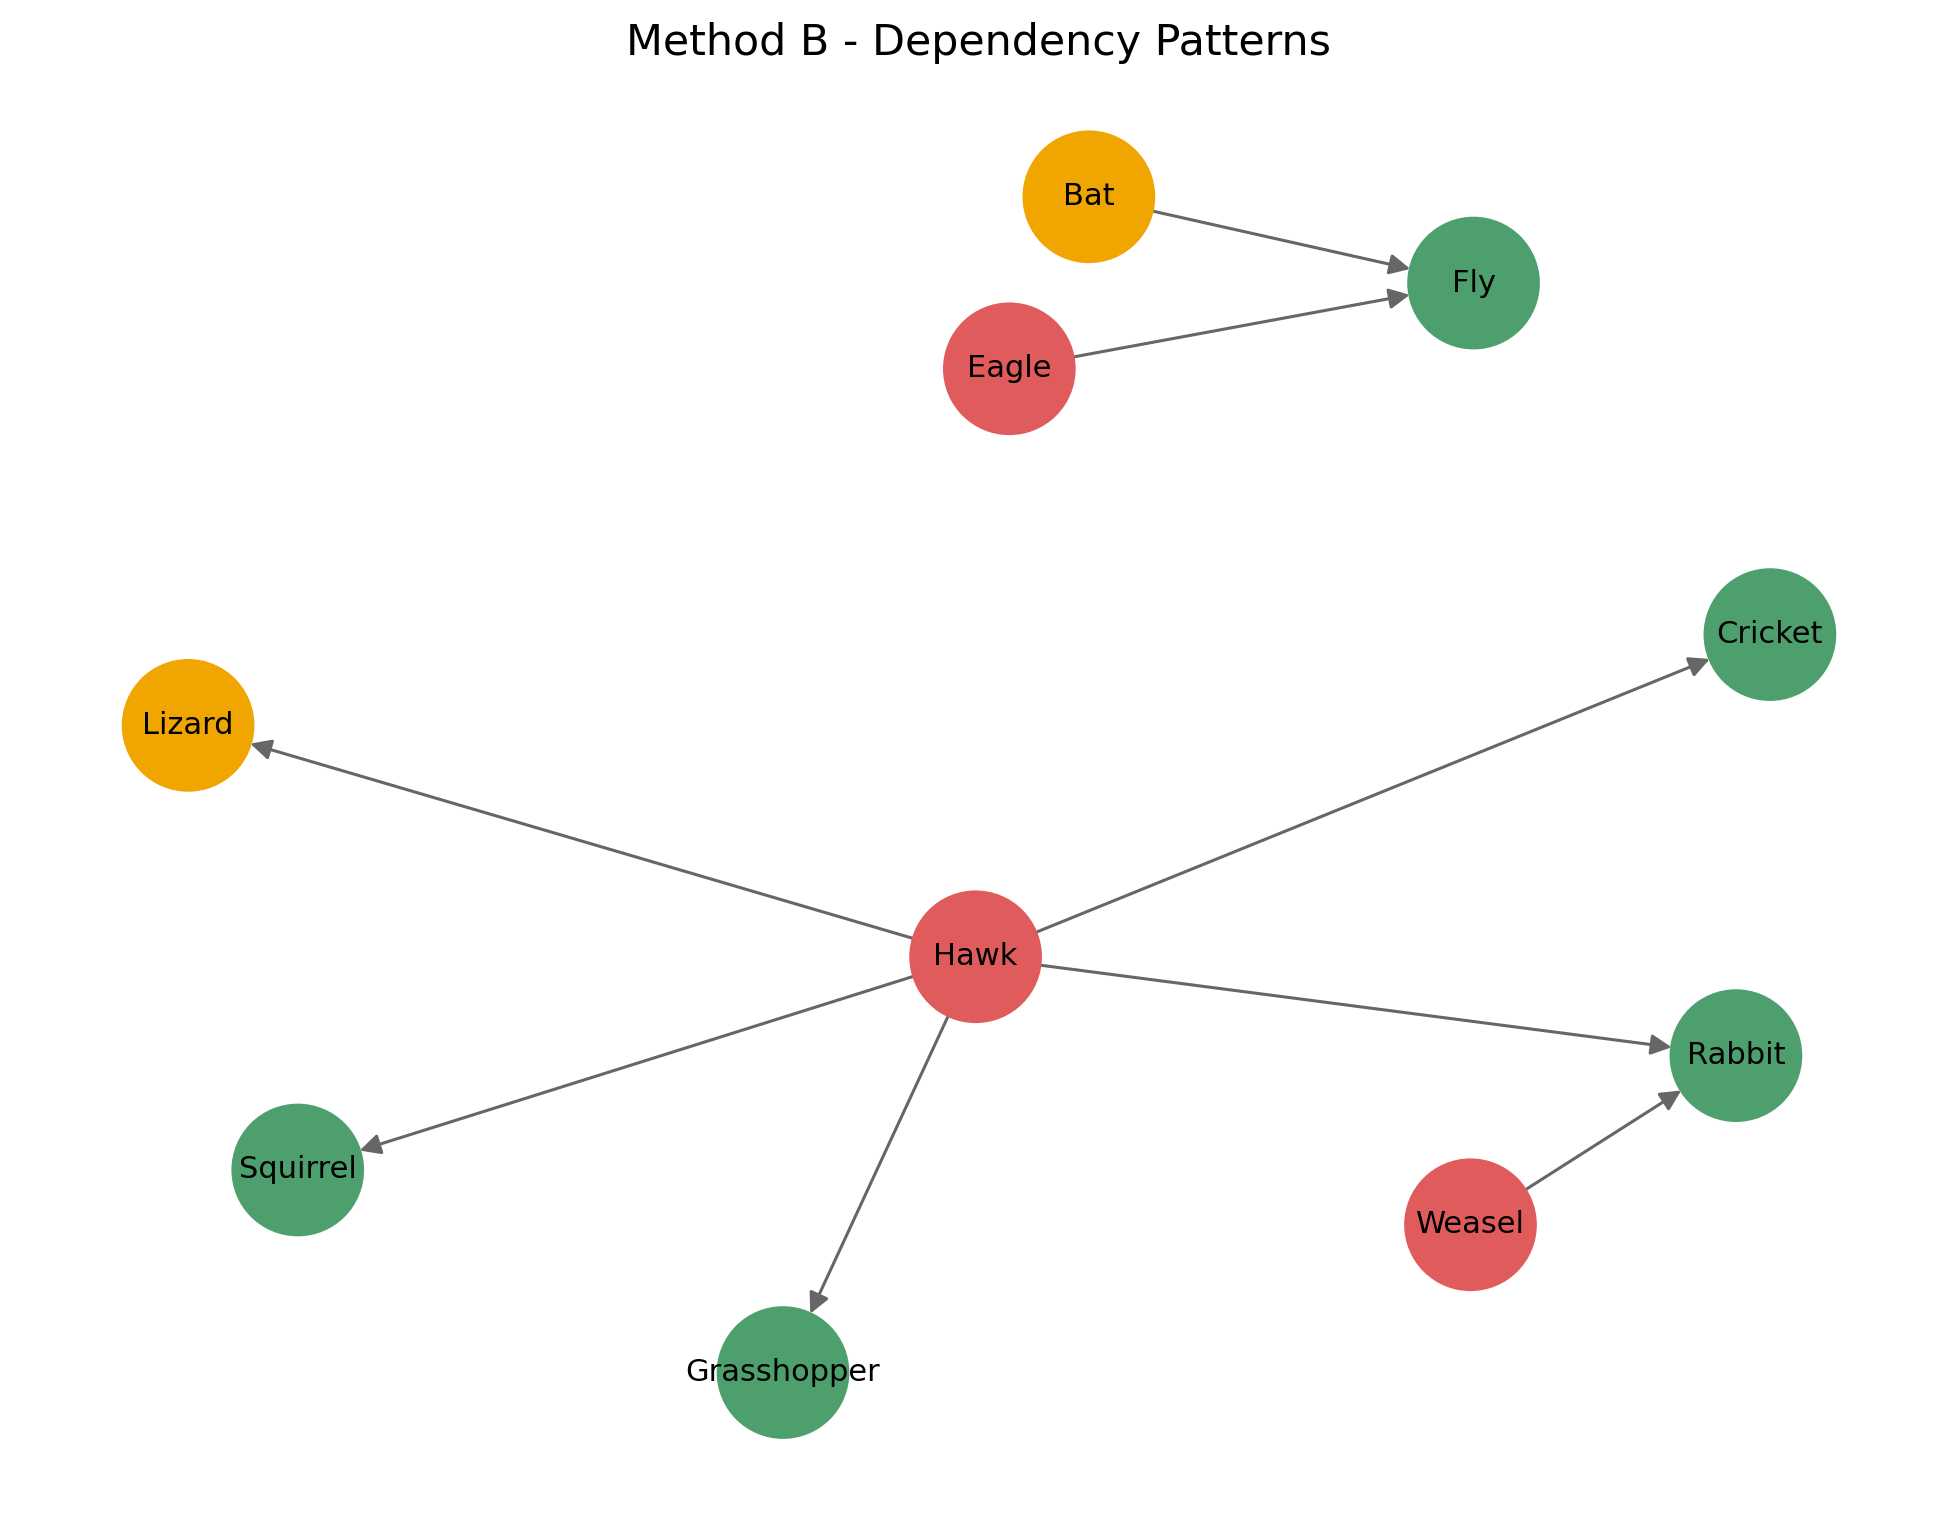
\includegraphics[width=\linewidth]{slides_assets/method_B_food_web.png}
  \end{columns}
  \vspace{0.4em}
  \begin{center}
    \small
    \textbf{Scores:} Precision $= 0.625$, Recall $= 0.139$, F1 $= 0.227$ \quad (TP $= 5$, FP $= 3$, FN $= 31$)
  \end{center}
\end{frame}

% ─── METHOD B ────────────────────────────────────────────────────────────────

\begin{frame}{Method B --- Predation Verb Patterns}
  \begin{twopanelrow}
    \twopanel{How it works}{
      \small
      \begin{enumerate}
        \item For each sentence containing the source animal, extract a window around both animals.
        \item Require at least one \alert{predation verb or phrase} inside that window:\\
              \emph{eats, feeds on, preys on, hunts, consumes, kills, devours,} \ldots
        \item \alert{Infer direction:}
          \begin{itemize}
            \item Active: ``Fox \emph{hunts} Rabbit'' $\to$ Fox$\to$Rabbit.
            \item Passive: ``Rabbit \emph{is hunted by} Fox'' $\to$ Fox$\to$Rabbit.
          \end{itemize}
        \item Per-source trophic constraints filter implausible edges.
      \end{enumerate}
    }
    \twopanel{Design trade-offs}{
      \small
      \good: the verb requirement dramatically reduces false positives
      compared to Method~A.

      \vspace{0.5em}
      \bad: paraphrased predation (\emph{``diet consists of\ldots''},
      \emph{``food source for\ldots''}) is missed, lowering recall.

      \vspace{0.5em}
      \bad: direction inference from text position is heuristic; complex
      sentence structures may be mis-directed.

      \vspace{0.5em}
      \bad: plural forms (mice, flies) not handled uniformly in the
      window search.

      \vspace{0.5em}
      \textbf{Expected:} highest precision, moderate recall.
    }
  \end{twopanelrow}
  \note{
    Method B is the precision anchor. It shows that insisting on an explicit
    verb is a necessary but not sufficient condition for high F1.
  }
\end{frame}

\begin{frame}{Method C vs Gold Standard}
  \begin{columns}[T,totalwidth=\textwidth]
    \column{0.49\textwidth}
      \centering
      \textbf{Gold standard}\\[0.3em]
      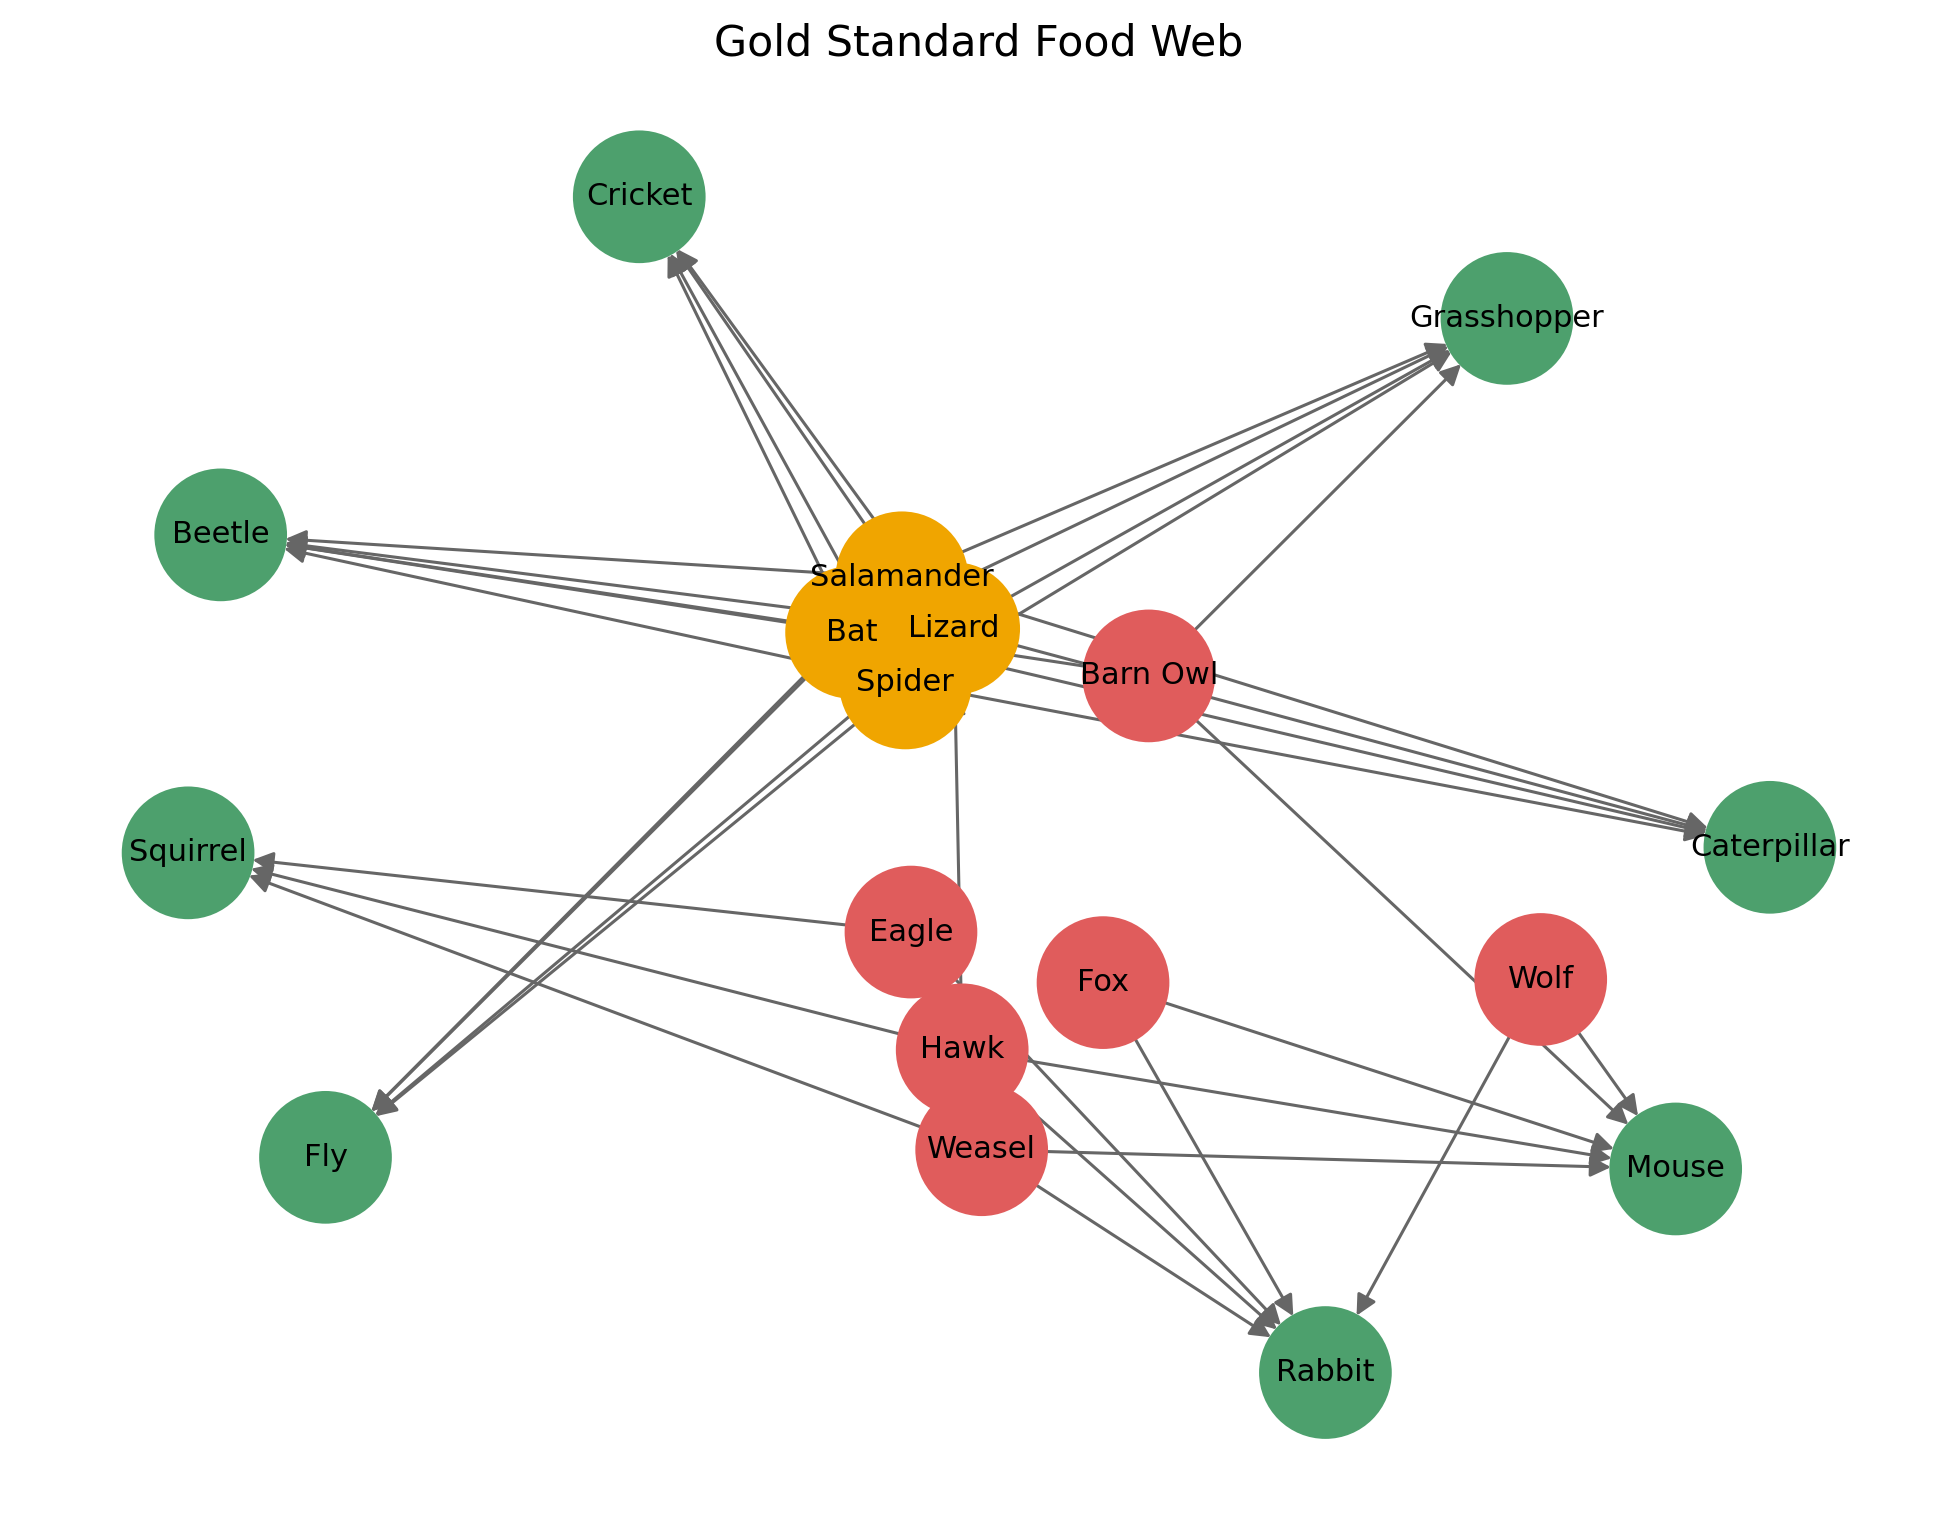
\includegraphics[width=\linewidth]{slides_assets/gold_standard_food_web.png}
    \column{0.49\textwidth}
      \centering
      \textbf{Method C}\\[0.3em]
      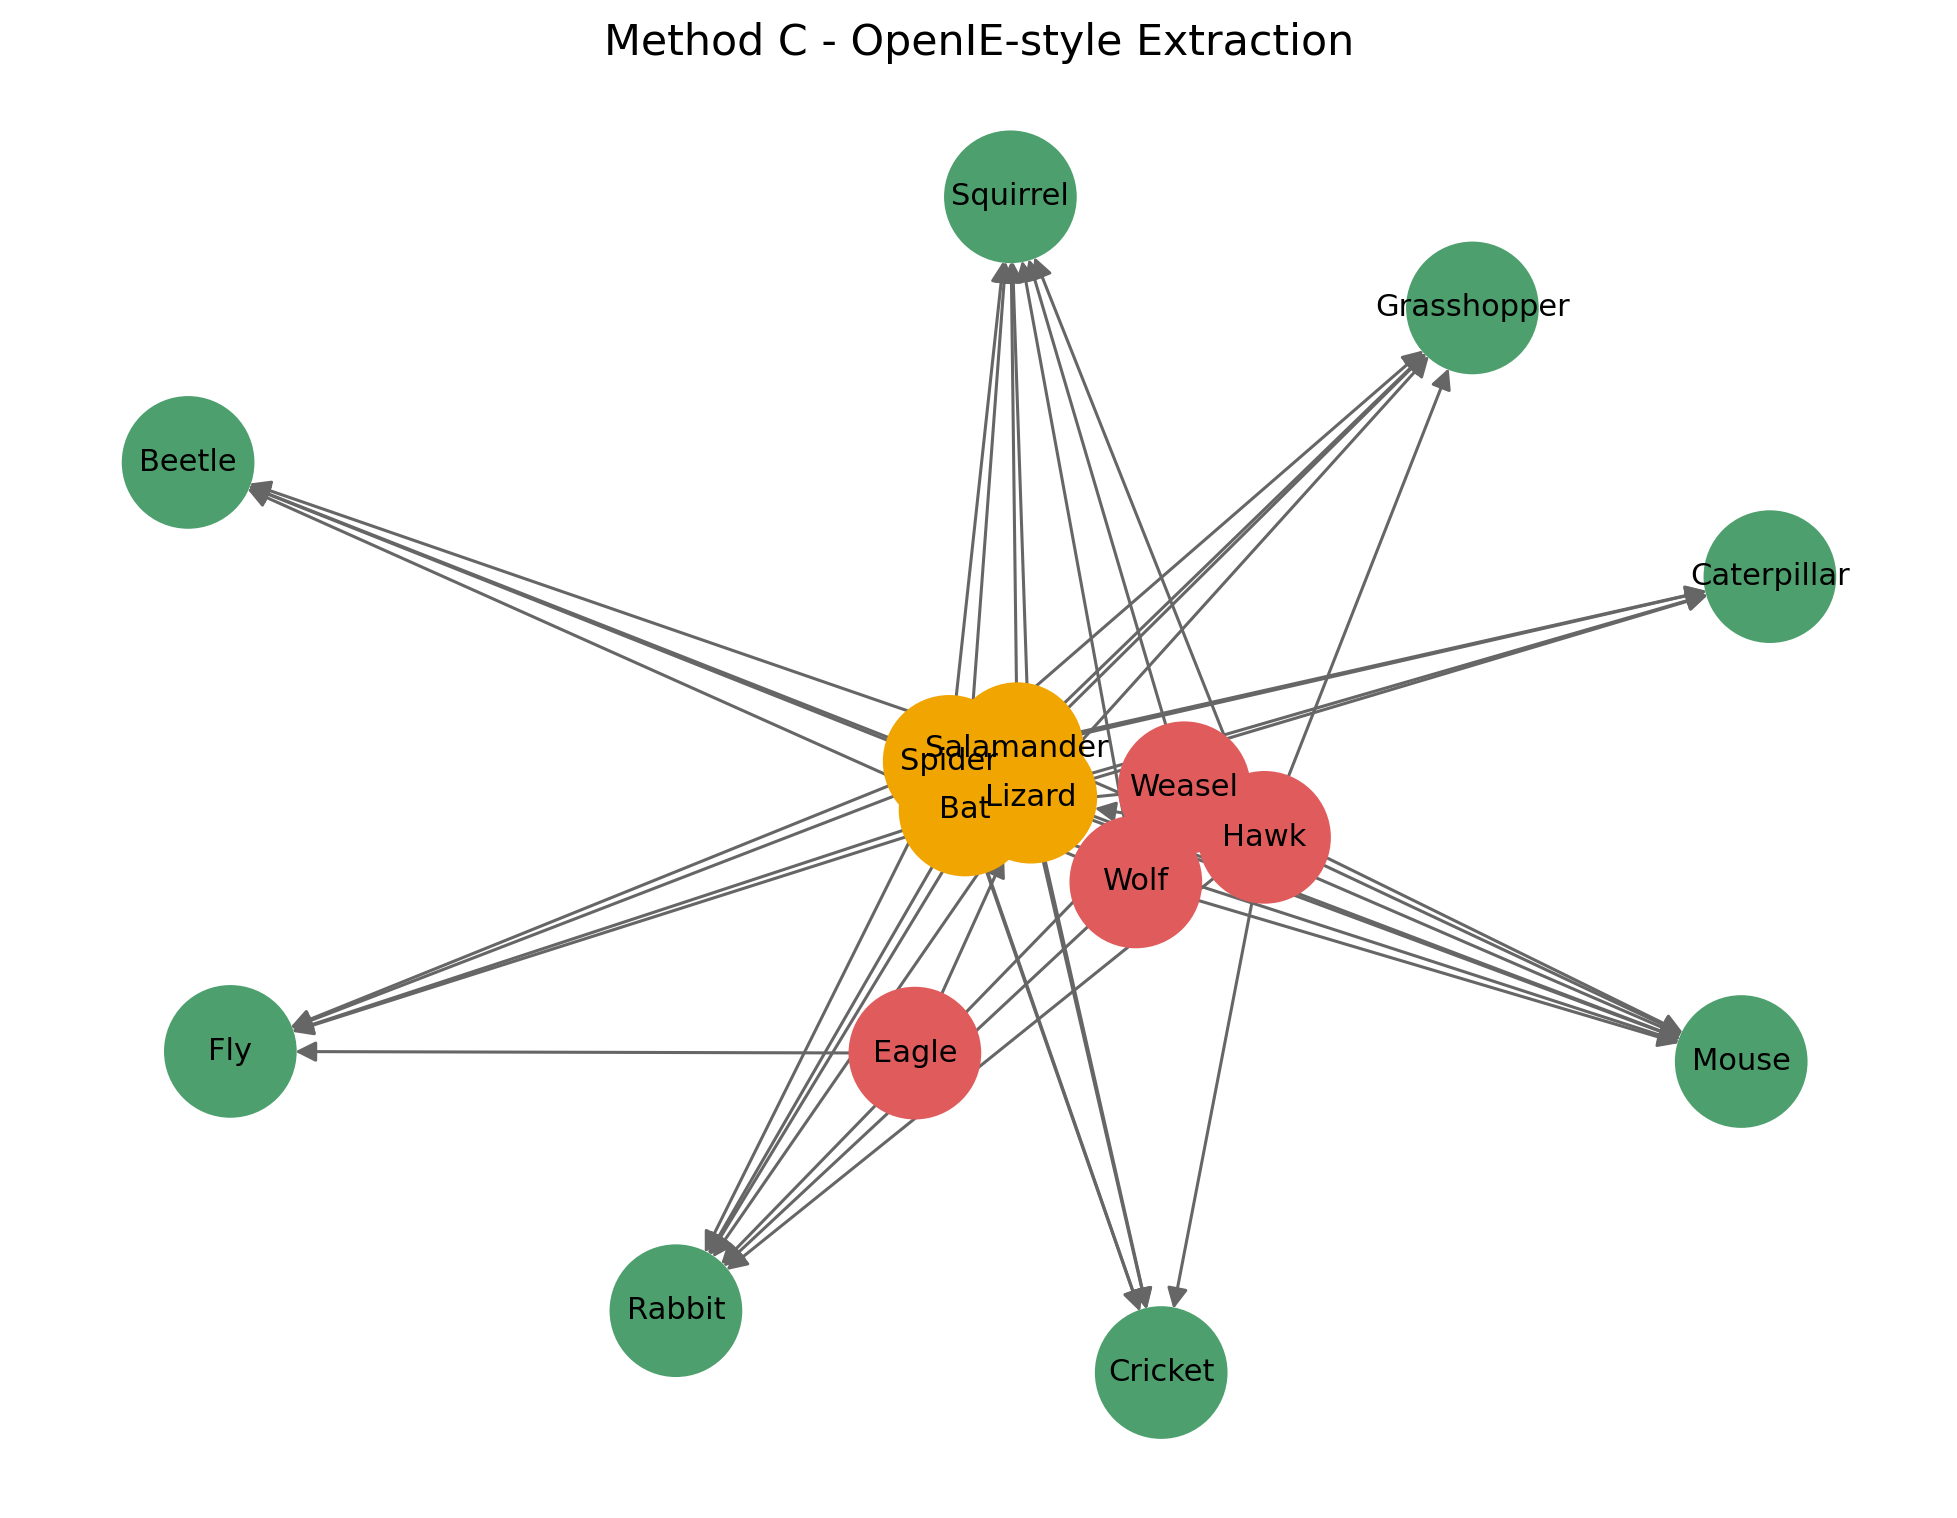
\includegraphics[width=\linewidth]{slides_assets/method_C_food_web.png}
  \end{columns}
  \vspace{0.4em}
  \begin{center}
    \small
    \textbf{Scores:} Precision $= 0.677$, Recall $= 0.583$, F1 $= 0.627$ \quad (TP $= 21$, FP $= 10$, FN $= 15$)
  \end{center}
\end{frame}

% ─── METHOD C ────────────────────────────────────────────────────────────────

\begin{frame}{Method C --- OpenIE-style Relation Extraction}
  \begin{columns}[T,totalwidth=\textwidth]
    \column{0.56\textwidth}
      \small
      \textbf{Core idea:} extract \texttt{(subject, relation, object)} triples.

      \vspace{0.4em}
      \begin{block}{Step-by-step}
        \begin{enumerate}
          \item Build regex from the full predation phrase + keyword vocabulary.
          \item Search for \texttt{[source] \ldots [rel] \ldots [target]} up to 180 characters apart.
          \item Handle passive: \texttt{[target] \ldots is eaten by \ldots [source]}.
          \item \alert{Noisy-context filter}: skip sentences with \emph{``such as'', ``food chain'', ``including'',} etc.\ unless a strong phrase is also present.
          \item \alert{Category expansion fallback}: if no explicit target is found but a sentence says ``eats insects'', expand to all insects in the corpus.
        \end{enumerate}
      \end{block}
    \column{0.40\textwidth}
      \small
      \good: variable-distance regex captures paraphrases missed by Method~B's fixed window.

      \vspace{0.5em}
      \good: category expansion recovers edges when Wikipedia mentions a category (``insects'') rather than a specific animal.

      \vspace{0.5em}
      \bad: generous distance windows may allow subject--relation--object triples that are not actually related.

      \vspace{0.5em}
      \bad: unconstrained category expansion can introduce false positives for all members of a category.

      \vspace{0.5em}
      \textbf{Expected:} better recall than B, moderate precision.
  \end{columns}
  \note{
    Emphasise the category expansion idea --- it is the main novel step over
    Method B, and the main source of both extra recall and extra false positives.
  }
\end{frame}

\begin{frame}{Method D vs Gold Standard}
  \begin{columns}[T,totalwidth=\textwidth]
    \column{0.49\textwidth}
      \centering
      \textbf{Gold standard}\\[0.3em]
      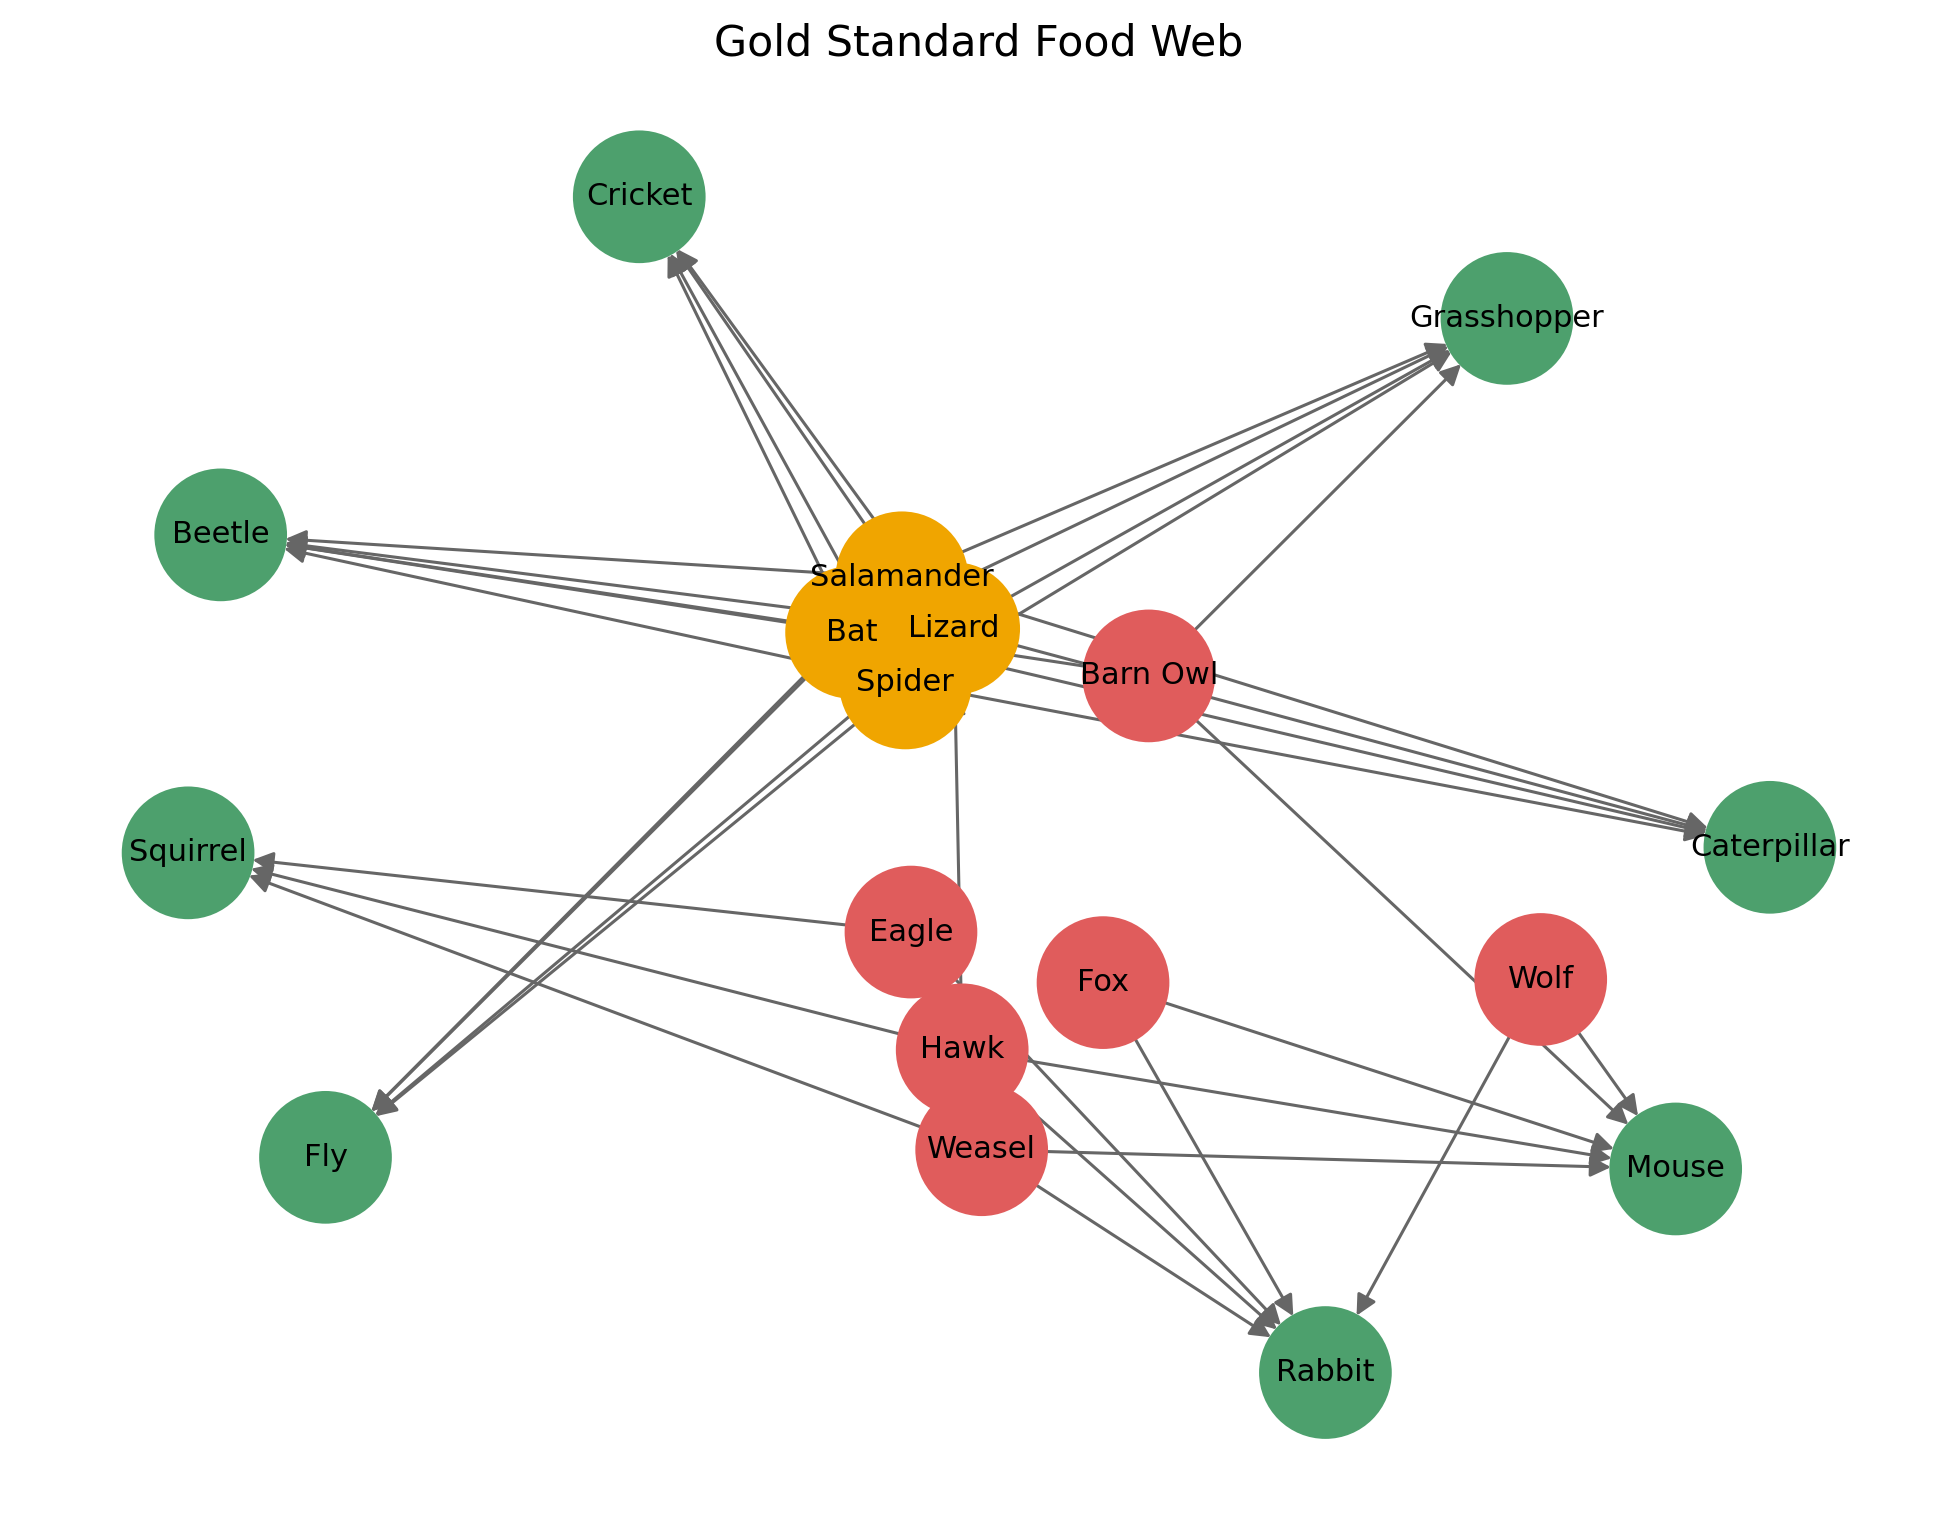
\includegraphics[width=\linewidth]{slides_assets/gold_standard_food_web.png}
    \column{0.49\textwidth}
      \centering
      \textbf{Method D}\\[0.3em]
      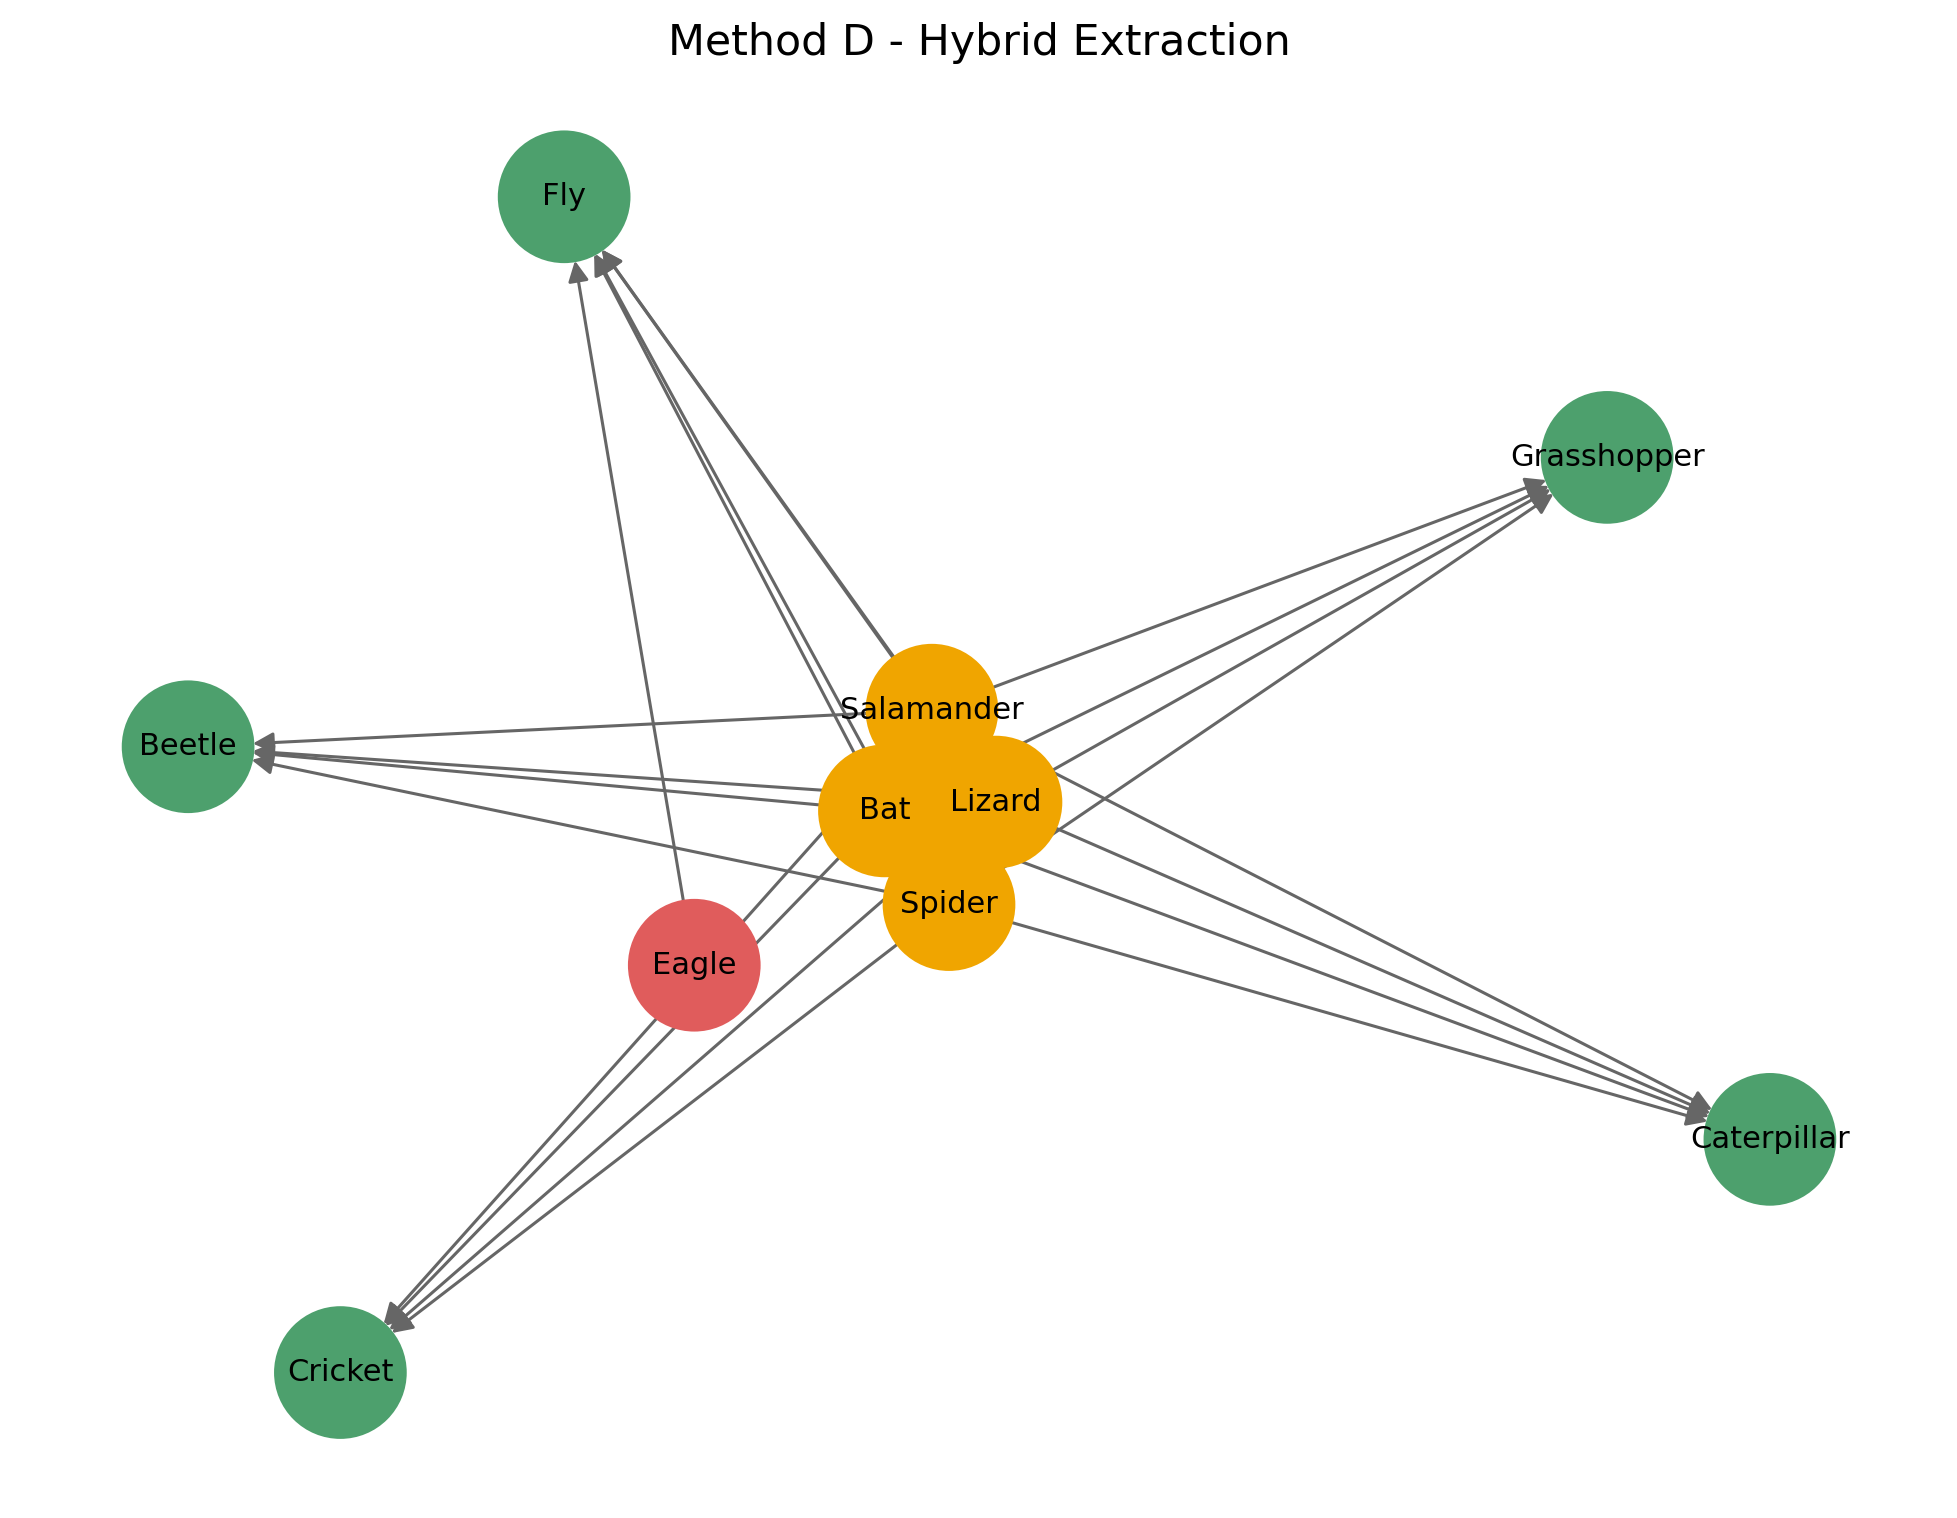
\includegraphics[width=\linewidth]{slides_assets/method_D_food_web.png}
  \end{columns}
  \vspace{0.4em}
  \begin{center}
    \small
    \textbf{Scores:} Precision $= 0.938$, Recall $= 0.417$, F1 $= 0.577$ \quad (TP $= 15$, FP $= 1$, FN $= 21$)
  \end{center}
\end{frame}

% ─── METHOD D ────────────────────────────────────────────────────────────────

\begin{frame}{Method D --- Hybrid Extraction}
  \begin{columns}[T,totalwidth=\textwidth]
    \column{0.56\textwidth}
      \small
      \textbf{Two-step pipeline per sentence:}
      \vspace{0.3em}
      \begin{block}{Step 1 --- Explicit verb proximity}
        \begin{itemize}
          \item Tokenise sentence; find strong predation verbs:\\
                \emph{eats, feeds on, preys on, hunts, consumes, devours}.
          \item For each target animal found: compute \alert{token distance} to the nearest verb.
          \item Add edge only if distance $\leq 8$ tokens.
          \item Variant matching: mice/mouse, flies/fly, etc.\ handled explicitly.
        \end{itemize}
      \end{block}
      \vspace{0.3em}
      \begin{block}{Step 2 --- Restricted category expansion}
        \begin{itemize}
          \item Triggered only when Step~1 adds nothing.
          \item Limited to insect prey and known insectivore sources\\
                (Salamander, Lizard, Spider, Bat).
        \end{itemize}
      \end{block}
    \column{0.40\textwidth}
      \small
      \good: token-distance gate (8 tokens) is stricter than Method~B/C windows, reducing false positives.

      \vspace{0.4em}
      \good: explicit variant matching avoids the plural-form gaps of Method~B.

      \vspace{0.4em}
      \bad: strict distance may miss relations that span a long noun phrase.

      \vspace{0.4em}
      \bad: restricted category expansion means mammal prey (Mouse, Rabbit) relies entirely on Step~1 explicit verbs.

      \vspace{0.4em}
      \good: passive constructions (e.g., ``is eaten by'') are handled in Step~1.

      \vspace{0.4em}
      \textbf{Expected:} best F1 --- a practical precision--recall balance.
  \end{columns}
  \note{
    Method D is the hybrid contribution of the project. Walk through both steps
    and explain why limiting category expansion to insectivores avoids the
    over-generation problem of Method~C.
  }
\end{frame}

% ─── DESIGN COMPARISON ───────────────────────────────────────────────────────

\begin{frame}{Method Design Comparison}
  \small
  \begin{center}
  \begin{tabular}{lcccc}
    \toprule
    & \textbf{A} Co-occurrence
    & \textbf{B} Verb patterns
    & \textbf{C} OpenIE
    & \textbf{D} Hybrid \\
    \midrule
    Predation verb required  & \textcolor{td3red}{No}   & \textcolor{td3green}{Yes} & \textcolor{td3green}{Yes}             & \textcolor{td3green}{Yes} \\
    Direction inference      & \textcolor{td3red}{No}   & \textcolor{td3green}{Yes} & \textcolor{td3green}{Yes}             & \textcolor{td3green}{Yes} \\
    Passive voice handled    & ---                      & \textcolor{td3green}{Yes} & \textcolor{td3green}{Yes}             & \textcolor{td3green}{Yes}   \\
    Category expansion       & \textcolor{td3red}{None} & \textcolor{td3red}{None}  & \textcolor{td3gold}{Full}             & \textcolor{td3green}{Restricted} \\
    Proximity constraint     & \textcolor{td3red}{None} & \textcolor{td3gold}{Window} & \textcolor{td3gold}{Char.\ distance} & \textcolor{td3green}{Token $\leq$8} \\
    Noisy-context filter     & \textcolor{td3red}{No}   & \textcolor{td3red}{No}    & \textcolor{td3green}{Yes}             & \textcolor{td3red}{No}   \\
    Variant matching         & \textcolor{td3green}{Yes}& \textcolor{td3red}{Partial}& \textcolor{td3green}{Yes}            & \textcolor{td3green}{Yes} \\
    \midrule
    Expected precision       & Low       & High          & Medium        & Medium-high \\
    Expected recall          & High      & Medium        & High          & Medium-high \\
    \bottomrule
  \end{tabular}
  \end{center}
  \note{
    Use this table as a summary before showing the numbers. It lets the audience
    predict the results before revealing them.
  }
\end{frame}

% ─── EVALUATION SETUP ────────────────────────────────────────────────────────

\begin{frame}{Evaluation Metrics}
  \begin{twopanelrow}
    \twopanel{Edge-level evaluation}{
      Let $\hat{E}$ be the set of predicted edges and $E^{*}$ the gold standard.
      \[
        \text{Precision} = \frac{|\hat{E} \cap E^{*}|}{|\hat{E}|}
        \qquad
        \text{Recall} = \frac{|\hat{E} \cap E^{*}|}{|E^{*}|}
      \]
      \[
        F_1 = \frac{2 \cdot P \cdot R}{P + R}
      \]
      \begin{itemize}
        \item $|\hat{E} \cap E^{*}|$ = true positives (TP)
        \item $|\hat{E}| - \text{TP}$ = false positives (FP)
        \item $|E^{*}| - \text{TP}$ = false negatives (FN)
      \end{itemize}
    }
    \twopanel{Scope constraint}{
      \small
      Only edges that satisfy the trophic direction are considered valid:
      \vspace{0.3em}
      \begin{itemize}
        \item Source must be in \textcolor{td3red}{top predators} $\cup$ \textcolor{td3gold}{mid-level}.
        \item Target must be in \textcolor{td3gold}{mid-level} $\cup$ \textcolor{td3green}{prey}.
        \item Self-loops are never valid.
        \item Top predators cannot appear as prey targets.
      \end{itemize}
      \vspace{0.3em}
      All four methods use this same constraint, implemented via \texttt{sanitize\_edges()}.
    }
  \end{twopanelrow}
  \note{
    Explain the scope constraint clearly. It is important for the audience
    to understand that we never penalise a method for not predicting biologically
    impossible edges.
  }
\end{frame}

% ─── RESULTS ─────────────────────────────────────────────────────────────────

\begin{frame}{Results}
  \begin{columns}[T,totalwidth=\textwidth]
    \column{0.52\textwidth}
      \small
      \begin{center}
      \begin{tabular}{lrrrrrr}
        \toprule
        \textbf{Method} & \textbf{P} & \textbf{R} & \textbf{F1} & \textbf{TP} & \textbf{FP} & \textbf{FN} \\
        \midrule
        A --- Co-occ.  & 0.556 & 0.278 & 0.370 & 10 & 8 & 26 \\[2pt]
        B --- Verb     & 0.625 & 0.139 & 0.227 & 5 & 3 & 31 \\[2pt]
        C --- OpenIE   & 0.677 & 0.583 & 0.627 & 21 & 10 & 15 \\[2pt]
        D --- Hybrid   & 0.938 & 0.417 & 0.577 & 15 & 1 & 21 \\
        \bottomrule
      \end{tabular}
      \end{center}
    \column{0.44\textwidth}
      \begin{block}{What to look for}
        \small
        \begin{itemize}
          \item \alert{High FP}: method is too lenient --- predicts edges not in gold.
          \item \alert{High FN}: method is too strict --- misses gold edges.
          \item \alert{F1} balances both; best method maximises it.
        \end{itemize}
      \end{block}
      \vspace{0.4em}
      \small
      \textbf{Expected ordering:}\\
      $\text{Recall}: \text{A} \geq \text{C} \geq \text{D} > \text{B}$\\
      $\text{Precision}: \text{B} \geq \text{D} \geq \text{C} > \text{A}$\\
      $\text{F1}: \text{D} \geq \text{C} \geq \text{B} > \text{A}$
  \end{columns}
  \note{
    If actual numbers are available, fill the table before the presentation.
    Otherwise walk through the expected ordering and explain the reasoning
    behind each prediction.
  }
\end{frame}

% ─── ERROR ANALYSIS ──────────────────────────────────────────────────────────

\begin{frame}{Error Analysis}
  \begin{threepanelrow}
    \threepanel{Method A --- False Positives}{
      \small
      Any co-occurrence becomes an edge:
      \begin{itemize}
        \item Taxonomic sentences:\\
              \emph{``Hawks and eagles are raptors.''}
        \item Competition sentences:\\
              \emph{``Foxes compete with wolves for rabbits.''}
        \item Encyclopedic lists:\\
              \emph{``Predators include hawks, owls, and foxes.''}
      \end{itemize}
    }
    \threepanel{Method B --- False Negatives}{
      \small
      Paraphrased predation is missed:
      \begin{itemize}
        \item \emph{``diet consists of\ldots''} not in the verb list.
        \item Inverted subject:\\\emph{``Grasshoppers are a major food source for lizards.''}
        \item Plurals (mice, flies) not matched by simple \texttt{str.find}.
        \item Indirect mention across sentence boundaries.
      \end{itemize}
    }
    \threepanel{Method D --- Residual gaps}{
      \small
      Strict token distance is conservative:
      \begin{itemize}
        \item Long noun phrases between verb and prey push distance $> 8$.
        \item Passive constructions are handled in Step~1.
        \item Category expansion restricted to insects --- mammal prey relies purely on explicit verbs.
      \end{itemize}
    }
  \end{threepanelrow}
  \note{
    Walk through one concrete sentence example for each method. Error analysis
    is often the most insightful part of an NLP evaluation.
  }
\end{frame}

% ─── DISCUSSION ──────────────────────────────────────────────────────────────

\begin{frame}{Discussion}
  \begin{twopanelrow}
    \twopanel{What we learned}{
      \small
      \begin{itemize}
        \item \alert{Co-occurrence (A)}: strong recall ceiling, but floods the graph with false edges --- not usable alone.
        \item \alert{Verb patterns (B)}: requiring a predation cue is \emph{necessary} for acceptable precision, but insufficient for high recall.
        \item \alert{OpenIE (C)}: category expansion helps when Wikipedia speaks at the category level (``eats insects''), but needs a noise filter.
        \item \alert{Hybrid (D)}: combining a strict proximity gate with restricted expansion is the most practical balance.
      \end{itemize}
    }
    \twopanel{Future directions}{
      \small
      \begin{itemize}
        \item \textbf{Coreference resolution}: link pronouns and nominals back to the subject.
        \item \textbf{Cross-page evidence}: if Rabbit's page says ``preyed on by foxes'', use that signal when building Fox's graph.
        \item \textbf{Pretrained RE models}: REBEL or similar models as a stronger neural baseline.
        \item \textbf{Larger gold standard}: independent annotation across more animal pairs to reduce gold-standard bias.
        \item \textbf{Ensemble}: take the intersection of B and C to combine high precision with broad recall.
      \end{itemize}
    }
  \end{twopanelrow}
  \note{
    Spend about two minutes here. The cross-page evidence point and the ensemble
    idea are the most practically interesting follow-ups.
  }
\end{frame}

% ─── SUMMARY ─────────────────────────────────────────────────────────────────

\begin{frame}{Summary}
  \small
  \begin{center}
  \begin{tabular}{clll}
    \toprule
    & \textbf{Method} & \textbf{Core signal} & \textbf{Best for} \\
    \midrule
    A & Co-occurrence  & sentence co-occurrence             & maximum recall       \\
    B & Verb patterns  & predation verb in window           & maximum precision    \\
    C & OpenIE         & regex triple + category expansion  & balanced recall      \\
    D & Hybrid         & verb proximity $\leq$ 8 tokens +   & best F1              \\
      &                & restricted expansion               &                      \\
    \bottomrule
  \end{tabular}
  \end{center}

  \vspace{0.6em}
  \begin{center}
    \normalsize
    Building knowledge graphs from free text requires \alert{balancing linguistic signal strength against coverage}.\\[0.4em]
    No single method dominates on all metrics ---
    \alert{hybrid approaches} that combine precision-oriented and recall-oriented signals are the most practical.
  \end{center}
  \note{
    Close by restating the central finding in one sentence: hybrid methods win.
    Leave time for questions.
  }
\end{frame}

% ─────────────────────────────────────────────────────────────────────────────
\end{document}
